\documentclass[12pt,a4paper,oneside]{report}

% =====================================================================
% BLACK BOOK DRAFT -- generated from the repository contents.
% Preamble is identical to Capstone_BlackBook_LaTeX_Template_REVISED/main.tex
% except for the clearly marked "DRAFT ADDITIONS" block below.
%
% Red   [MISSING: ...] = required by the template, not found in the repo.
% Orange [VERIFY: ...] = found in the repo, but needs your confirmation.
% See MISSING_AND_FLAGS.md for the full list.
% =====================================================================

% ---------- Page layout and typography ----------
\usepackage[a4paper,left=1.5in,right=1in,top=1in,bottom=1in]{geometry}
\usepackage{newtxtext,newtxmath} % Times-like text and math font
\usepackage{setspace}
\onehalfspacing
\usepackage{indentfirst}
\setlength{\parindent}{0.5in}
\setlength{\parskip}{0pt}
\usepackage{titlesec}
\titleformat{\chapter}[display]
  {\normalfont\bfseries\centering\fontsize{16}{19}\selectfont}
  {\MakeUppercase{\chaptername\ \thechapter}}{10pt}{\MakeUppercase}
\titlespacing*{\chapter}{0pt}{-10pt}{24pt}
\titleformat{\section}
  {\normalfont\bfseries\fontsize{14}{17}\selectfont}
  {\thesection}{1em}{}
\titleformat{\subsection}
  {\normalfont\bfseries\fontsize{12}{14}\selectfont}
  {\thesubsection}{1em}{}
\titleformat{\subsubsection}
  {\normalfont\bfseries\itshape\fontsize{12}{14}\selectfont}
  {\thesubsubsection}{1em}{}

% ---------- Figures, tables, references, and links ----------
\usepackage{graphicx}
\usepackage{float}
\usepackage{booktabs}
\usepackage{array}
\usepackage{tabularx}
\usepackage{longtable}
\usepackage{caption}
\captionsetup{font=small,labelfont=bf}
\usepackage{amsmath}
\usepackage{url}
\usepackage[hidelinks]{hyperref}
\usepackage[numbers,sort&compress]{natbib}
\usepackage{enumitem}
\usepackage{listings}
\usepackage{xcolor}
\usepackage{chngcntr}
\counterwithin{figure}{chapter}
\counterwithin{table}{chapter}
\numberwithin{equation}{chapter}

\lstset{
  basicstyle=\ttfamily\small,
  breaklines=true,
  frame=single,
  numbers=left,
  numberstyle=\tiny,
  captionpos=b
}

% ---------- DRAFT ADDITIONS (not in the original template) ----------
\usepackage{tikz}
\usepackage{pgfgantt}
% Running header and chapter divider pages, following "Capstone_BB Format_2026-27.docx.pdf"
\usepackage{fancyhdr}
\setlength{\headheight}{15pt}
% Running header: short form of the title (the full title does not fit on one header line)
\newcommand{\HeaderTitle}{Do the Numbers Hold on Real Hardware?}
% List label spacing
\setlist[enumerate]{labelsep=0.5em,leftmargin=2.4em}
\setlist[itemize]{labelsep=0.5em,leftmargin=2.4em}
\fancypagestyle{fancy}{\fancyhf{}\fancyhead[R]{\footnotesize\HeaderTitle}\fancyfoot[C]{\thepage}\renewcommand{\headrulewidth}{0.6pt}}
\fancypagestyle{plain}{\fancyhf{}\fancyhead[R]{\footnotesize\HeaderTitle}\fancyfoot[C]{\thepage}\renewcommand{\headrulewidth}{0.6pt}}
\pagestyle{fancy}
\newcommand{\ChapterDivider}[1]{%
  \clearpage\thispagestyle{empty}\null\vfill
  \begin{center}{\large\bfseries CHAPTER: \number\numexpr\value{chapter}+1\relax}\\[1.2in]{\large\bfseries\MakeUppercase{#1}}\end{center}
  \vfill\null\clearpage}
\usetikzlibrary{positioning,shapes.geometric,shapes.multipart,fit,calc,arrows}
\setlength{\emergencystretch}{3em}
\newcolumntype{Y}{>{\raggedright\arraybackslash}X}
\newcolumntype{P}[1]{>{\raggedright\arraybackslash}p{#1}}
\newcommand{\MISSING}[1]{\textcolor{red}{\textbf{[MISSING: #1]}}}
\newcommand{\VERIFY}[1]{\textcolor{orange!85!black}{\textbf{[VERIFY: #1]}}}
\tikzset{
  every picture/.append style={execute at begin picture={\linespread{1}\selectfont}},
  blk/.style={draw,rounded corners=2pt,align=center,minimum height=8mm,inner sep=4pt,font=\small},
  grp/.style={draw,dashed,rounded corners=4pt,inner sep=6pt},
  arr/.style={-latex,thick},
  proc/.style={draw,circle,align=center,minimum size=20mm,font=\footnotesize,inner sep=1pt},
  ext/.style={draw,rectangle,align=center,minimum height=9mm,minimum width=22mm,font=\footnotesize},
  store/.style={draw,rectangle,align=center,minimum height=7mm,font=\footnotesize,
                path picture={\draw (path picture bounding box.north west) -- (path picture bounding box.south west);}},
  usecase/.style={draw,ellipse,align=center,font=\footnotesize,minimum width=36mm,minimum height=9mm},
  cls/.style={draw,rectangle split,rectangle split parts=3,align=left,font=\scriptsize,text width=33mm}
}

% ---------- Report details: replace all placeholders ----------
\newcommand{\ProjectTitle}{Do the Numbers Hold on Real Hardware? A Reproducibility and Measurement Audit of a Low-Cost Hybrid ECC Authentication Protocol for IoT}
\newcommand{\StudentNames}{Jay Kerkar, Chaitanya Kelkar, Chirag Poornamath and Yash Kolekar}
\newcommand{\StudentRollNos}{16, 15, 26, 17}
% Names and guide: CITATION.cff, README.md and paper/main.tex
\newcommand{\GuideName}{Dr.\ Shanta Sondur}
\newcommand{\DepartmentName}{Department of Information Technology}
\newcommand{\InstituteName}{Vivekanand Education Society's Institute of Technology}
\newcommand{\AcademicYear}{2026--2027}

\begin{document}

% ==================== TITLE PAGE (layout of the Format PDF) ====================
\begin{titlepage}
\begin{center}
\vspace*{-0.4in}

\includegraphics[width=1.15in]{figures/logos/mu_emblem.png}\\[0.15in]
{\large\bfseries \ProjectTitle\par}
\vspace{0.12in}
{\normalsize ON\par}
\vspace{0.12in}
{\normalsize Submitted in partial fulfillment of the requirements of\\ the degree of\par}
\vspace{0.1in}
{\large\bfseries Bachelor of Engineering\par}
\vspace{0.05in}
{\normalsize\bfseries (Information Technology)\par}
\vspace{0.12in}
{\normalsize By\par}
\vspace{0.06in}
{\normalsize\bfseries Jay Kerkar -- Roll No. 16\par}
{\normalsize\bfseries Chaitanya Kelkar -- Roll No. 15\par}
{\normalsize\bfseries Chirag Poornamath -- Roll No. 26\par}
{\normalsize\bfseries Yash Kolekar -- Roll No. 17\par}
\vspace{0.12in}
{\normalsize Under the guidance of\par}
\vspace{0.05in}
{\normalsize\bfseries \GuideName\par}
\vspace{0.15in}

\includegraphics[width=0.75in]{figures/logos/vesit_logo.png}\\[0.1in]
{\normalsize\bfseries \DepartmentName\par}
{\normalsize\bfseries VIVEKANAND EDUCATION SOCIETY'S INSTITUTE OF TECHNOLOGY,\\ Chembur, Mumbai 400074\par}
{\normalsize\bfseries (An Autonomous Institute, Affiliated to University of Mumbai)\par}
\vspace{0.12in}
{\normalsize\bfseries AY (2026-27)\par}
\end{center}
\end{titlepage}

% ==================== PRELIMINARY PAGES ====================
\pagenumbering{roman}
\setcounter{page}{1}

\clearpage
\thispagestyle{empty}
\addcontentsline{toc}{chapter}{Certificate}
\begin{center}
\vspace*{-0.5in}

\includegraphics[width=\textwidth]{figures/logos/ves_letterhead.png}\\[0.25in]
{\LARGE\bfseries\itshape Certificate\par}
\vspace{0.15in}
This is to certify that project entitled\\[0.05in]
{\bfseries ``\ProjectTitle''\par}
\vspace{0.2in}
{\bfseries Group Members Names\par}
\vspace{0.05in}
Jay Kerkar (Roll No. 16)\\
Chaitanya Kelkar (Roll No. 15)\\
Chirag Poornamath (Roll No. 26)\\
Yash Kolekar (Roll No. 17)\\[0.2in]
In partial fulfilment of the Fourth Year (Sem.\ VI--Sem.\ VII), Bachelor of Engineering (B.E.) Degree in Information Technology at the University of Mumbai\\[0.15in]
Academic Year 2026-27
\end{center}

\vspace{0.6in}
\noindent
\begin{tabular}{@{}>{\centering\arraybackslash}p{0.47\textwidth}>{\centering\arraybackslash}p{0.47\textwidth}@{}}
\textbf{\GuideName} & \textbf{External Examiner}\\
\textbf{Project Mentor} & \\[0.7in]
\textbf{Dr.\ (Mrs.)\ Shalu Chopra} & \textbf{Dr.\ (Mrs.)\ J.\,M.\ Nair}\\
\textbf{H.O.D} & \textbf{Principal}\\
\end{tabular}

\vspace{0.5in}
\noindent Date: \quad / \quad /2026\\
Place:\\
VESIT, Chembur \hfill College Seal

\chapter*{Declaration}
\addcontentsline{toc}{chapter}{Declaration}
We hereby declare that the project report entitled \textbf{\ProjectTitle} is our original work carried out as part of the Semester VII Capstone Project. The work has been completed under the guidance of \GuideName. All sources of information used in this report have been appropriately acknowledged and cited. This report has not been submitted, in whole or in part, for any other degree or qualification.

\vspace{0.8in}
\noindent
\begin{tabular}{p{0.42\textwidth}p{0.42\textwidth}}
Name: Jay Kerkar & Name: Chaitanya Kelkar\\[0.15in]
Roll No.: 16 & Roll No.: 15\\[0.4in]
Signature: \rule{1.5in}{0.4pt} & Signature: \rule{1.5in}{0.4pt}\\[0.5in]
Name: Chirag Poornamath & Name: Yash Kolekar\\[0.15in]
Roll No.: 26 & Roll No.: 17\\[0.4in]
Signature: \rule{1.5in}{0.4pt} & Signature: \rule{1.5in}{0.4pt}
\end{tabular}

\chapter*{Acknowledgement}
\addcontentsline{toc}{chapter}{Acknowledgement}
The project report on \textbf{\ProjectTitle} is the outcome of the guidance, moral support and devotion bestowed on our group throughout our work. We express our sincere gratitude to Dr.\ (Mrs.)\ Shalu Chopra, Head of the Department of Information Technology \VERIFY{name/designation}, to \MISSING{Deputy HOD name and designation, if to be included}, and to our project guide \GuideName, for their valuable inputs, consistent guidance and support. We also thank Vivekanand Education Society's Institute of Technology for providing a stimulating atmosphere and a conducive work environment, including institutional access to the IEEE Xplore digital library through which the base paper for this project was obtained.

\MISSING{Any other individuals or organisations the group wishes to thank.}

\chapter*{Abstract}
\addcontentsline{toc}{chapter}{Abstract}
Internet of Things (IoT) devices and servers must authenticate each other before exchanging data over shared wireless channels, and the authentication must be cheap enough for constrained devices. Al-Rasheed \emph{et al.}\ (IEEE Transactions on Consumer Electronics, 2026) propose a hybrid protocol that uses elliptic curve cryptography only in an offline registration phase and a two-message symmetric-key handshake online. They report about 17\%, 21\% and 12\% lower communication, processing and storage cost than prior schemes, based on simulation and assumed per-operation times. This project implements the protocol and tests those claims. A Python reference implementation follows the paper's nonce-based model, because its narrative algorithm is replayable. It passes 108 tests with 97\% coverage, including 10{,}000 key-agreement trials and eight adversarial cases. A C port of the device side runs on an ESP8266 microcontroller and interoperates with the Python server, costing 5.26~ms of computation per handshake. Measuring the underlying primitives with one benchmark on the ESP8266, an AWS Graviton2 core and a laptop shows that an ECC scalar multiplication takes 276~ms on the ESP8266, sixteen times the assumed value, while symmetric operations are five to twelve times faster than assumed. With these measured constants, the protocol is 60 to 2{,}500 times cheaper than the ECC-based schemes it is compared with. However, it costs more than the verified hash-only schemes once the session-key derivation required by its own equations is counted. A consistency audit finds that the paper's headline percentages cannot be derived from its own tables or figures, and its simulated processing figure cannot be reproduced from published information. The protocol also lacks forward secrecy, and its server-side pseudonym lookup grows with the number of devices. A field test on two cloud instances found three implementation weaknesses that a deployment would need to fix.

\vspace{0.2in}
\noindent\textbf{Keywords:} Internet of Things, Mutual Authentication, Elliptic Curve Cryptography, Reproducibility, Microcontroller Benchmarking, Lightweight Security

\tableofcontents
\listoffigures
\addcontentsline{toc}{chapter}{List of Figures}
\listoftables
\addcontentsline{toc}{chapter}{List of Tables}

\chapter*{List of Abbreviations}
\addcontentsline{toc}{chapter}{List of Abbreviations}
\begin{tabular}{lp{0.75\textwidth}}
AAD & Additional Authenticated Data\\
AEAD & Authenticated Encryption with Associated Data\\
AES & Advanced Encryption Standard\\
CI & Continuous Integration\\
CLI & Command-Line Interface\\
CSPRNG & Cryptographically Secure Pseudo-Random Number Generator\\
DFD & Data Flow Diagram\\
ECC & Elliptic Curve Cryptography\\
ECDH & Elliptic Curve Diffie--Hellman\\
GCM & Galois/Counter Mode\\
HKDF & HMAC-based Key Derivation Function\\
IoT & Internet of Things\\
KDF & Key Derivation Function\\
MAC & Message Authentication Code (or Media Access Control address, by context)\\
MCU & Microcontroller Unit\\
NIST & National Institute of Standards and Technology\\
PID & Pseudonymous Identifier\\
PoC & Proof of Concept\\
PPT & Probabilistic Polynomial Time\\
PRD & Product Requirements Document\\
SHA & Secure Hash Algorithm\\
TA & Trusted Authority\\
TCP & Transmission Control Protocol\\
UML & Unified Modeling Language\\
\end{tabular}

% ==================== MAIN REPORT ====================
\clearpage
\pagenumbering{arabic}
\setcounter{page}{1}

\ChapterDivider{Introduction}
\chapter{Introduction}
\section{Introduction}
The Internet of Things (IoT) connects sensors, actuators, appliances and other embedded systems that sense their environment, exchange data with nearby devices and servers, and act on what they receive \cite{alrasheed2026hybrid}. These devices usually communicate over shared wireless channels, so an adversary on the same channel can eavesdrop, replay earlier messages, inject forged ones, or impersonate a legitimate server. Before a device and a server exchange application data, each must therefore confirm that the other is a trusted participant. This is called \emph{mutual authentication}.

Lightweight authentication schemes for IoT are usually compared by counting the cryptographic operations each party performs and multiplying by an assumed time per operation. The result of such a comparison then depends on a few constants that are rarely measured on the kind of device the scheme targets \cite{kerkar2026audit}. Al-Rasheed \emph{et al.}\ \cite{alrasheed2026hybrid} propose a hybrid scheme in which elliptic curve cryptography (ECC) is used only in an offline registration phase run by a Trusted Authority (TA), and every online authentication uses a two-message, nonce-based symmetric handshake. Using an OMNeT++ simulation and assumed per-operation times, they report about 17\%, 21\% and 12\% lower communication, processing and storage cost than prior schemes.

This project takes that paper as its base. It first turns the protocol into working, tested software: a Python reference implementation and a C port of the device side that runs on an ESP8266 microcontroller. It then uses that software to check the paper's claims: it audits the paper's tables and figures for consistency, measures the cryptographic primitives on real hardware, recomputes the paper's cost model with the measured values, and examines security properties the paper does not discuss. The results were written up by the team as a manuscript \cite{kerkar2026audit}.

\section{Problem Definition}
At the start of the project the protocol existed only as a paper description that had been validated in simulation. As recorded in the project's requirements document (PRD, v0.1, 25 August 2026), there was no way to:
\begin{enumerate}[nosep]
  \item confirm that the protocol can be implemented as specified without hidden ambiguities;
  \item verify its claimed security properties with concrete, executable tests; or
  \item validate the paper's quantitative claims against an independent, code-based measurement rather than a simulator.
\end{enumerate}
Two further problems emerged while working on the paper. First, its evidence cannot be re-run: the simulation behind its figures has no published code, scenario or data, and its cost tables rely on assumed constants (e.g.\ 17.1~ms for an ECC scalar multiplication) that were never measured on IoT hardware. Second, the paper describes the online phase twice. The narrative algorithm in Section~II reuses a static digest across sessions and is therefore replayable. The mathematical model in Section~III uses fresh nonces and is the version the paper's security sketch covers. An implementation must choose one and justify the choice.

These problems matter to security reviewers who need a concrete artefact to audit, to researchers who want to compare against the scheme, and to engineers deciding whether the scheme is worth deploying on constrained devices.

\section{Objectives}
The first group of objectives comes from the PRD (goals G1--G7 and its acceptance criteria). The second group was added when the project was extended into a measurement-based audit; it follows the contributions listed in the team's manuscript \cite{kerkar2026audit}.

\textbf{Implementation objectives.}
\begin{enumerate}[nosep]
  \item Implement offline TA registration, pseudonym derivation and the two-message mutual authentication of Section~III as a tested Python library, with at least 90\% line coverage on the \path{protocol/} and \path{crypto/} packages.
  \item Verify session-key agreement (Eq.~\ref{eq:correct}) in at least 10{,}000 randomised trials with zero failures.
  \item Provide TA, device and server command-line tools that run a complete registration and authentication on one machine, including a visible, correctly classified rejection of a replayed message.
  \item Implement and pass eight adversarial test cases (SEC-01 to SEC-08).
  \item Measure communication, processing and storage cost on real code, and complete one authentication in under 5~ms median (excluding network) on a laptop CPU.
\end{enumerate}

\textbf{Measurement and audit objectives.}
\begin{enumerate}[nosep,resume]
  \item Port the device side to C and run it on a microcontroller (ESP8266) against the unmodified Python server.
  \item Measure the primitives the paper's cost model uses (hash, symmetric encryption, ECC scalar multiplication, KDF) on the ESP8266, a cloud ARM core and a laptop, using one C source on every platform.
  \item Audit the paper's tables, equations and figures for internal consistency, and check its competitor rows against the original papers where available.
  \item Recompute the paper's cost model with the measured constants, and state for each claim whether it is supported.
  \item Attempt to reproduce the paper's simulated processing figure (Fig.~1), and report honestly what can and cannot be reproduced.
\end{enumerate}

\section{Motivation}
Three observations motivated this work. First, IoT authentication must be cheap: constrained devices cannot afford heavy asymmetric cryptography or multi-message handshakes on every session, and the paper's design targets exactly this constraint. Second, lightweight schemes have a history of being broken after publication. Chang and Le \cite{chang2016provably} showed that the scheme of Turkanovi\'{c} \emph{et al.}\ \cite{turkanovic2014novel} is vulnerable to several attacks, and Jiang \emph{et al.}\ \cite{jiang2016robust} showed comparable flaws in an earlier three-factor scheme. A protocol that has only been simulated deserves an executable implementation before anyone relies on it. Third, the paper's conclusions depend on assumed constants. If a scalar multiplication or an encryption costs very different amounts on a real microcontroller, the ranking of schemes can change, so the constants themselves have to be measured.

\section{Scope of the Work}
\textbf{In scope.}
\begin{itemize}[nosep]
  \item A Python package (\texttt{hybrid\_ecc\_auth}) with cryptographic wrappers, the TA, device and server state machines, a versioned wire format, replay and block-list bookkeeping, an optional login pre-check, command-line demonstrations over TCP, a benchmark harness and a test suite with continuous integration.
  \item A portable C device core and ESP8266 (NodeMCU) firmware that interoperate with the Python server, plus a C primitive benchmark.
  \item A two-node field test of the Python implementation on AWS t4g.nano instances.
  \item A consistency audit of the base paper, a recomputation of its cost model with measured constants, protocol-level checks (forward secrecy, server lookup cost), an attempted reproduction of its Fig.~1, and a replication of its competitor rows and simulation environment, including an OMNeT++ model used as a sensitivity analysis.
\end{itemize}

\textbf{Intended users} (from the PRD): security reviewers and auditors, applied-cryptography researchers, product-engineering teams evaluating a production version, and firmware teams who may port the protocol.

\textbf{Out of scope.}
\begin{itemize}[nosep]
  \item Production hardening: no hardware security module, no formal verification (ProVerif or Tamarin), no penetration test, no side-channel protection.
  \item Device mobility and hand-off; devices are treated as static, as in the paper.
  \item TA-assisted rekeying (Eq.~24 of the paper), which is a stub only.
  \item Re-implementing the nine competitor protocols; their costs are the paper's operation counts multiplied by measured times.
  \item 8- and 16-bit microcontrollers, MCUs with cryptographic hardware, and energy measurement.
  \item Running the Section~II ECDH registration exchange; the TA derives secrets locally as in Eq.~8.
\end{itemize}

\section{Feasibility Study}
\textbf{Technical feasibility.} All primitives the protocol needs (NIST P-256, SHA-256, HKDF-SHA256, AES-256-GCM) are available in the open-source \texttt{cryptography} library \cite{pyca_cryptography} for Python and in BearSSL \cite{bearssl}, which ships with the ESP8266 Arduino core. Feasibility has been demonstrated in practice: the full test suite and the paper-scale benchmark run in seconds on a laptop, the C device core completes handshakes on an ESP8266 over Wi-Fi, and the protocol ran between two cloud instances (Chapter~4).

\textbf{Operational feasibility.} The demonstration needs three terminals on one machine and a single \texttt{pip install -e .}. The ESP8266 firmware is built and flashed with PlatformIO, and a native build of the same C core can be checked against the Python server without hardware.

\textbf{Economic feasibility.} All software used is free or open source. Hardware consists of laptops, two NodeMCU ESP8266 boards and short-lived AWS t4g.nano instances, which the AWS demo report prices at US\$0.0042 per hour each. The base paper was obtained through the institute's IEEE Xplore access. \MISSING{Prices of the ESP8266 boards, the AWS bill in rupees, and whether the laptops are personally owned or institute-provided.}

\section{Organization of the report}
Chapter~2 reviews the literature on lightweight IoT mutual authentication, including the base paper and the comparator papers whose full texts were studied, and sets out the research gaps. Chapter~3 presents the methodology: requirements, the protocol algorithms, the cost-model recomputation, the project timeline, architecture and UML diagrams, hardware and software requirements, and cost estimation. Chapter~4 describes the implementation (Python, C/ESP8266, cloud test, audit and replication tooling) and presents and analyses the results. Chapter~5 gives limitations, conclusions and future scope. The appendix holds publication and competition details.

\ChapterDivider{Literature Survey}
\chapter{Literature Survey}
\section{Introduction}
This survey examines how existing IoT mutual authentication schemes balance security against communication, computation and storage overhead, and locates the base paper \cite{alrasheed2026hybrid} within that landscape. Because this project also audits the base paper's comparison, the survey pays particular attention to the comparator schemes the base paper evaluates: what they actually compute, which time constants their own authors used, and whether the base paper transcribed them correctly. The sources are peer-reviewed journal and conference papers: the base paper, three comparator papers whose full texts were studied (Dhillon and Kalra; Chang and Le; Jiang \emph{et al.}), and further schemes cited by the base paper, which are described from secondary sources only.

\section{Review of Literature Survey}

\subsection*{Paper 1}
\noindent\textbf{Title:} A Low-Cost Hybrid Elliptic Curve Cryptography Authentication Protocol for Trustworthy Internet of Things Communication\\
\textbf{Link:} \url{https://doi.org/10.1109/TCE.2026.3662053}\\
\textbf{Authors and year:} A.~Al-Rasheed, R.~Khan, A.~Ahmad, A.~Saeed, F.~Alturise and S.~Alkhalaf, 2026 \cite{alrasheed2026hybrid}.

\noindent\textbf{Summary.} The paper addresses mutual authentication between IoT devices and servers over shared channels. A Trusted Authority registers every device and server offline, deriving a per-entity secret $\lambda_X = H_1(ID_X \| s) \bmod n$ and distributing the secrets of trusted peers. Online, a device and server derive a pairwise symmetric root key and authenticate each other with two messages: an encrypted challenge carrying a rotating pseudonym and a fresh nonce, and an encrypted response carrying the server's nonce, after which both derive a session key. The scheme block-lists an entity after three failed attempts and conditions communication on radio coverage. It is evaluated by OMNeT++ simulation and by operation counts multiplied by assumed constants (Table~III) against nine prior schemes.

\noindent\textbf{Observations.} (i) Online, only a KDF, symmetric encryption and a MAC are used (Eq.~22). (ii) The abstract reports about 17\%, 21\% and 12\% lower communication, processing and storage cost. (iii) The Section~II algorithm and the Section~III model describe different protocols; only Section~III uses per-session nonces. (iv) The cost constants are assumed, not measured. (v) The paper contains internal inconsistencies: Table~IV lists the proposed scheme with 4 messages and 1{,}024 bits, the text says 2 messages and 264 bits; Section~V names OMNeT++ while the conclusion names SUMO; Table~II lists a 160~km/h speed for supposedly static devices; and several comparator labels in Tables~IV--V point to the wrong entries in its own reference list. (vi) No simulation code, scenario or data is published.

\noindent\textbf{Inference drawn.} The Section~III model is implementable and its security sketch can be turned into tests, but the quantitative claims rest on evidence that cannot be re-run. The paper therefore needs both an implementation and an independent, measurement-based check. It is the base paper of this project.

\subsection*{Paper 2}
\noindent\textbf{Title:} A lightweight biometrics based remote user authentication scheme for IoT services\\
\textbf{Link:} \url{https://doi.org/10.1016/j.jisa.2017.01.003}\\
\textbf{Authors and year:} P.~K.~Dhillon and S.~Kalra, 2017 \cite{dhillon2017lightweight}.

\noindent\textbf{Summary.} A multi-factor (password, smart device, biometric) remote user authentication and key agreement scheme. A user registers through a gateway node and then connects directly to a sensor node. Only one-way hashes, perceptual hashes and XOR operations are used.

\noindent\textbf{Observations.} Security is argued against multiple attacks and verified formally with AVISPA. Computation is very low because there are no encryption or ECC operations. The paper gives no per-operation time constants of its own, only that a hash value is 128 bits. Its Table~3 tabulates Turkanovi\'{c} \emph{et al.}\ at 7/5/7 hash operations for user, sensor node and gateway. The authors leave a testbed evaluation on real devices to future work.

\noindent\textbf{Inference drawn.} A hash-only scheme can be cheaper to compute than a scheme that uses symmetric encryption and a KDF. This paper is one of the two independent sources that confirm the base paper's hash-only comparator rows, and it also shows the base paper's Turkanovi\'{c} row has device and server counts swapped.

\subsection*{Paper 3}
\noindent\textbf{Title:} A Provably Secure, Efficient, and Flexible Authentication Scheme for Ad hoc Wireless Sensor Networks\\
\textbf{Link:} \url{https://doi.org/10.1109/TWC.2015.2473165}\\
\textbf{Authors and year:} C.-C.~Chang and H.-D.~Le, 2016 \cite{chang2016provably}.

\noindent\textbf{Summary.} The paper cryptanalyses the smart-card scheme of Turkanovi\'{c} \emph{et al.}\ and proposes two replacements: P1, which uses only hash and XOR operations, and P2, an ECC-based variant with perfect forward secrecy.

\noindent\textbf{Observations.} Turkanovi\'{c} \emph{et al.}'s scheme is shown vulnerable to impersonation with node capture, stolen smart cards, sensor-node spoofing and stolen verifiers, and to lack backward secrecy. Security of P1 and P2 is proven in the random oracle model. The authors use $t_h = 0.5$~ms and $t_{mul} = 63.075$~ms. The team's replication found that one printed cell (P2's user cost) does not match the paper's own constants. The base paper's row labelled ``Cheng and Le [14]'' matches P2 with the user and gateway hash counts exchanged, while its reference [14] points to a different paper (Wang \emph{et al.}, VANETs).

\noindent\textbf{Inference drawn.} The paper shows the trade-off between per-session ECC (forward secrecy, higher cost) and hash-only operation. The base scheme avoids per-session ECC entirely, so it cannot provide forward secrecy; this project tested that directly.

\subsection*{Paper 4}
\noindent\textbf{Title:} Robust extended chaotic maps-based three-factor authentication scheme preserving biometric template privacy\\
\textbf{Link:} \url{https://doi.org/10.1007/s11071-015-2467-5}\\
\textbf{Authors and year:} Q.~Jiang, F.~Wei, S.~Fu, J.~Ma, G.~Li and A.~Alelaiwi, 2016 \cite{jiang2016robust}.

\noindent\textbf{Summary.} The paper shows that Islam's chaotic-map three-factor scheme has an invalid password check, is vulnerable to impersonation and off-line password guessing when the smart card is lost, and fails to protect the biometric template. It proposes a robust replacement and proves mutual authentication with BAN logic.

\noindent\textbf{Observations.} The scheme is \emph{not} hash-only. Its authentication phase costs $7T_H + 4T_C$ and login plus authentication cost $11T_H + 6T_C$, with the authors' own constants $T_H = 0.20$~ms and $T_C = 32.40$~ms. The base paper's Table~III sets $T_C = T_H = 0.32$~ms, about 100 times lower. The base paper's row labelled ``Jiang et al.\ [15]'' (7/5/10 hash operations) does not match this paper. A 2025 survey \cite{zhong2025lightweight} lists a different, two-factor scheme by Jiang \emph{et al.}\ \cite{jiang2015twofactor} at those counts, which is the likely source.

\noindent\textbf{Inference drawn.} The constants a comparison uses can decide its outcome. With its own $T_C$, this scheme becomes far more expensive than the base scheme, whereas the base paper's constants make it look cheaper. Comparator rows must be traced to their sources before conclusions are drawn from them.

\subsection*{Paper 5}
\noindent\textbf{Title:} A novel user authentication and key agreement scheme for heterogeneous ad hoc wireless sensor networks, based on the Internet of Things notion\\
\textbf{Link:} \MISSING{DOI/URL -- not in repo}\\
\textbf{Authors and year:} M.~Turkanovi\'{c}, B.~Brumen and M.~H\"{o}lbl, 2014 \cite{turkanovic2014novel}.

\noindent\VERIFY{The full text of this paper is not in the repository. This entry relies on the base paper, the team's literature survey, and the two papers that tabulate it (Chang and Le; Dhillon and Kalra). Please read the original and revise, or replace it with a paper whose full text you have.}

\noindent\textbf{Summary.} A smart-card-based user authentication and key agreement scheme for heterogeneous ad hoc wireless sensor networks in an IoT setting, using only hash and XOR operations.

\noindent\textbf{Observations.} It is the cheapest scheme in the base paper's Table~V. Chang and Le and Dhillon and Kalra both tabulate it at 7/5/7 hash operations (user/sensor/gateway); the base paper prints 7/7/5, swapping device and server. Chang and Le later showed it to be insecure, and it provides no forward secrecy.

\noindent\textbf{Inference drawn.} The cheapest scheme in a cost table may not be secure, so cost alone cannot rank schemes. Because its operation counts are confirmed by two independent papers, it is the cleanest hash-only comparator for the base scheme.

% Comparative summary table included within Section 2.2, without adding an extra index heading.
\begin{table}[H]
\centering
\caption{Comparative Summary of Literature Survey}
\label{tab:lit}
\small
\begin{tabularx}{\textwidth}{|>{\centering\arraybackslash}p{0.055\textwidth}|P{0.14\textwidth}|Y|P{0.17\textwidth}|Y|Y|}
\hline
\textbf{Sr. No.} & \textbf{Author(s), Year} & \textbf{Paper Title} & \textbf{Methodology / Technology} & \textbf{Key Observations} & \textbf{Inference Drawn}\\ \hline
1 & Al-Rasheed \emph{et al.}, 2026 & Low-cost hybrid ECC authentication protocol for trustworthy IoT & Offline ECC (TA); online KDF, AES-GCM, MAC; 2 messages; OMNeT++ & Claims 17/21/12\% savings; assumed constants; inconsistent tables; no published simulation & Implementable; claims need measurement-based checking\\ \hline
2 & Dhillon \& Kalra, 2017 & Lightweight biometrics-based remote user authentication for IoT services & Hash, perceptual hash, XOR; gateway; AVISPA & Very low computation; formally verified; no time constants & Hash-only scheme; confirms Turkanovi\'{c} counts\\ \hline
3 & Chang \& Le, 2016 & Provably secure, efficient, flexible authentication for ad hoc WSNs & Hash/XOR (P1), ECC (P2); random oracle proofs & Breaks Turkanovi\'{c}; P2 has forward secrecy; base paper's ``Cheng--Le'' row is P2 & Base scheme lacks forward secrecy\\ \hline
4 & Jiang \emph{et al.}, 2016 & Robust extended chaotic maps-based three-factor authentication & Chebyshev chaotic maps, smart card, biometrics; BAN logic & $T_C = 32.40$~ms, not 0.32~ms; not the base paper's ``Jiang'' row & Constants decide rankings; trace rows to sources\\ \hline
5 & Turkanovi\'{c} \emph{et al.}, 2014 & User authentication and key agreement for heterogeneous ad hoc WSNs & Smart card, hash, XOR & Cheapest in Table~V; later broken; device/server counts swapped in base paper & Cost alone is not sufficient\\ \hline
\end{tabularx}
\end{table}

The base paper also compares or cites the schemes in Table~\ref{tab:lit2}. Their descriptions come from the base paper, the team's survey document and the team's manuscript; their full texts are not in the repository.

\begin{table}[H]
\centering
\caption{Further schemes cited by the base paper (secondary-source descriptions)}
\label{tab:lit2}
\small
\begin{tabularx}{\textwidth}{|>{\centering\arraybackslash}p{0.055\textwidth}|P{0.2\textwidth}|P{0.24\textwidth}|Y|}
\hline
\textbf{Sr. No.} & \textbf{Author(s), Year} & \textbf{Mechanism} & \textbf{Limitation / note}\\ \hline
6 & Zong \emph{et al.}, 2024 \cite{zong2024relac} & Blockchain, revocable access control (ReLAC) & Revocation needs key regeneration or re-encryption\\ \hline
7 & Nawaz Khan \emph{et al.}, 2024 \cite{khan2024enabling} & Distributed public/private-key scheme & Overly complex for large networks\\ \hline
8 & Gong \emph{et al.}, 2023 \cite{gong2023lcdma} & Binary symmetric polynomials (LCDMA) & Cross-domain key distribution complexity\\ \hline
9 & Alshawish \& Al-Haj, 2022 \cite{alshawish2022efficient} & Hash + AES, six messages & Lengthy exchange\\ \hline
10 & Qiu \emph{et al.}, 2025 \cite{qiu2025lightweight} & Blockchain, medical IoT & Ledger overhead on low-power nodes\\ \hline
11 & Yin \& Gong, 2024 \cite{yin2024lightweight} & Certificateless signatures & Per-session signature overhead\\ \hline
12 & Sharma \& Dhiman, 2024 \cite{sharma2024secure} & Hash + XOR addressing & Centralised gateway\\ \hline
13 & Porambage \emph{et al.}, 2014 \cite{porambage2014two} & Two-phase ECC authentication & Most expensive row in Table~V\\ \hline
14 & Sadhukhan \emph{et al.}, 2021 \cite{sadhukhan2021lightweight} & ECC remote user authentication & Per-session ECC\\ \hline
15 & Challa \emph{et al.}, 2017 \cite{challa2017secure} & Signature-based key establishment & Shares reference [17] with the ``Wazid'' row in the base paper\\ \hline
16 & Fakroon \emph{et al.}, 2020 \cite{fakroon2020secure} & Anonymous remote user authentication & Bit total confirmed by \cite{banerjee2020efficient}\\ \hline
17 & Shuai \emph{et al.}, 2019 \cite{shuai2019anonymous} & Smart-home anonymous authentication, hash + ECC & Likely source of the ``Shuai [16]'' row, via \cite{banerjee2020efficient}; base paper adds one device ECC operation\\ \hline
18 & Jiang \emph{et al.}, 2015 \cite{jiang2015twofactor} & Two-factor WSN authentication, hash-only & Likely source of the ``Jiang [15]'' row, via \cite{zhong2025lightweight}\\ \hline
\end{tabularx}
\end{table}

\section{Research gaps}
Table~\ref{tab:gap} combines the gaps listed in the team's literature survey document with those found while implementing and auditing the base paper.

\begin{table}[H]
\centering
\caption{Research Gap Analysis}
\label{tab:gap}
\small
\begin{tabularx}{\textwidth}{|>{\centering\arraybackslash}p{0.055\textwidth}|P{0.2\textwidth}|Y|Y|}
\hline
\textbf{Sr. No.} & \textbf{Existing Approach / System} & \textbf{Identified Limitation / Research Gap} & \textbf{Proposed Project's Approach}\\ \hline
1 & Base paper & No implementation; validated only in simulation & Python reference implementation and an ESP8266 C device port that interoperate\\ \hline
2 & Base paper, Section~II & Static digest reused across sessions; replayable & Implement the Section~III nonce-based model; test replay rejection\\ \hline
3 & Base paper, Table~III & Per-operation times assumed, never measured on IoT hardware & Measure primitives on ESP8266, Graviton2 and a laptop with one C source\\ \hline
4 & Base paper, Tables~IV--VI and abstract & Headline percentages not derived; tables contradict text & Systematic consistency audit under nine definitions of ``reduction''\\ \hline
5 & Base paper, Table~V & Comparator rows not traceable; session KDF omitted from own count & Check rows against original papers; recompute with four readings (V1--V4)\\ \hline
6 & Base paper, Fig.~1 & Simulation has no published code, scenario or data & Attempted reproduction; own OMNeT++ model as sensitivity analysis only\\ \hline
7 & Base paper, Section~III & Epoch handling unspecified; forward secrecy and server lookup cost not discussed & Documented epoch window; tested forward secrecy and lookup scaling\\ \hline
8 & Base paper; most comparators & No machine-checked security proof & Executable adversarial tests only; formal verification left as future work\\ \hline
9 & Base paper; ReLAC & Static devices; single TA; no lightweight revocation & Not addressed; future work\\ \hline
\end{tabularx}
\end{table}

The central gap is the evidence gap in rows~3--6. The base paper's ranking of schemes depends on per-operation constants that were never measured, on comparator rows that cannot all be traced to their sources, and on a simulation that cannot be re-run. Until these are checked, neither the scheme's advantages nor its disadvantages are known. An implementation (rows~1--2) is the prerequisite for measuring anything, which is why the project builds it first and then uses it for the audit.

\VERIFY{The team's literature survey names mobility support and key revocation as the planned ``delta'' extensions, and the manuscript lists completing ``the TA-assisted key-revocation extension we proposed earlier'' as future work. The repository contains no revocation code. Confirm that the audit replaced the revocation extension as the project's main contribution.}

\section{Conclusion}
The surveyed schemes trade security against overhead in different ways. Blockchain- and certificate-based designs are strong but expensive. Hash/XOR and chaotic-map designs are cheap but have repeatedly been broken. ECC-per-session designs give forward secrecy at a higher computational cost. The base paper's hybrid design is a promising middle ground. However, the comparison that supports it uses unmeasured constants and partly untraceable comparator rows, and it cannot be re-run. The survey of the three comparator papers already shows that their own constants and operation counts differ from those the base paper used. These findings motivate the methodology in Chapter~3: implement the protocol, measure its primitives on real hardware, and recompute the comparison with evidence that can be checked.

\ChapterDivider{Proposed Methodology}
\chapter{Proposed Methodology}
\section{Introduction}
The project proceeds in four stages, shown in Figure~\ref{fig:workflow}. \textbf{Implement:} build a transport-agnostic Python implementation of the base paper's Section~III protocol, with demonstration tools, tests and a benchmark harness, following the eight phases of the PRD (cryptographic core; TA and registration; pseudonyms and login gate; mutual-authentication core; security hardening; benchmarking of the proposed scheme; baseline data and report; documentation, CI and release). Then port the device side to C and run it on an ESP8266 against the unmodified Python server. \textbf{Measure:} time the primitives the paper's cost model uses on the ESP8266, an AWS Graviton2 core and a laptop, with one C source and checksum-verified outputs. \textbf{Audit:} check the paper's tables, equations and figures for consistency, and trace its comparator rows to the original papers. \textbf{Recompute:} re-evaluate the paper's cost model with the measured constants, under several readings of the proposed scheme's cost, and use a separately written OMNeT++ model only as a sensitivity analysis. The implementation stage makes the measurements possible, and the measurements and audit address the evidence gap identified in Chapter~2.

\begin{figure}[H]
\centering
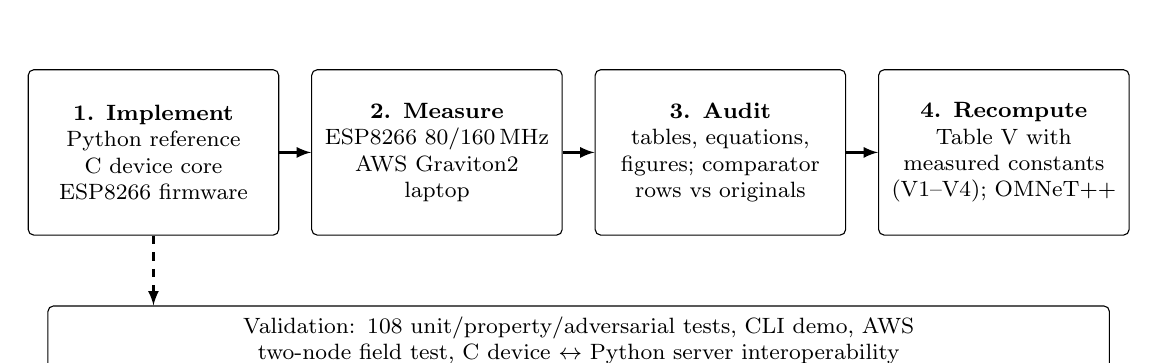
\begin{tikzpicture}[node distance=4mm]
\tikzset{wf/.style={blk,text width=29mm,minimum height=21mm,font=\footnotesize,anchor=north}}
\node[wf] (a) at (0,0) {\textbf{1. Implement}\\ Python reference\\ C device core\\ ESP8266 firmware};
\node[wf] (b) at (3.6,0) {\textbf{2. Measure}\\ ESP8266 80/160\,MHz\\ AWS Graviton2\\ laptop};
\node[wf] (c) at (7.2,0) {\textbf{3. Audit}\\ tables, equations,\\ figures; comparator\\ rows vs originals};
\node[wf] (d) at (10.8,0) {\textbf{4. Recompute}\\ Table~V with\\ measured constants\\ (V1--V4); OMNeT++};
\draw[arr] (a.east) -- (b.west); \draw[arr] (b.east) -- (c.west); \draw[arr] (c.east) -- (d.west);
\node[blk,text width=132mm,font=\footnotesize,anchor=north] (e) at (5.4,-3.0) {Validation: 108 unit/property/adversarial tests, CLI demo, AWS two-node field test, C device $\leftrightarrow$ Python server interoperability};
\draw[arr,dashed] (a.south) -- (a.south |- e.north);
\end{tikzpicture}
\caption{Overall project workflow}
\label{fig:workflow}
\end{figure}

\section{Requirement Gathering}
Requirements came from two sources. The first was a detailed study of the base paper: its equations (Eq.~8--24), algorithms, threat model, instantiation notes and evaluation tables, together with the comparator schemes reviewed in Chapter~2. The results were written up as a Product Requirements Document (PRD, Draft v0.1, 25 August 2026). The PRD records the decision to implement Section~III rather than Section~II, defines functional, non-functional, benchmarking and security requirements with identifiers (FR, NFR, BR, SEC) that the code and tests reference, and sets acceptance criteria. The second source was the project review cycle. The audit notes record a mentor's condition that the paper's Fig.~1 be reproduced (``their benchmark/dataset, or a model resolving to the same numbers'') before measured hardware results are compared with it; this led to the reproduction attempt and the replication study in Chapter~4. \VERIFY{The PRD says the Section~III decision was ``confirmed with stakeholders'', and the audit notes mention a ``mentor''. Add the actual review meetings, guide inputs or other requirement-gathering techniques used.}

\subsection{Functional Requirements}
\begin{table}[H]
\centering
\caption{Functional requirements (from the PRD) and implementation status}
\label{tab:fr}
\small
\begin{tabularx}{\textwidth}{|P{0.1\textwidth}|Y|P{0.2\textwidth}|}
\hline
\textbf{ID} & \textbf{Requirement} & \textbf{Status}\\ \hline
FR-1 & Primitives: NIST P-256; SHA-256 for $H_{1,2,3}$; HKDF-SHA256; AES-256-GCM (tag as MAC); CSPRNG nonces of 128 bits (192/256 configurable) & Implemented (\path{crypto/})\\ \hline
FR-2 & Offline TA: $\lambda_X = H_1(ID_X\|s) \bmod n$; optional $P_X=\lambda_X G$; no network I/O; batch enrolment from a manifest & Implemented (\texttt{ta.py}); no-socket invariant tested\\ \hline
FR-3 & Pairwise root $k^\star_{ij}=\mathrm{KDF}(\lambda_{V_i}\|\lambda_{R_j})$ on both sides, with caching and an invalidation hook & Implemented (\texttt{entity.py})\\ \hline
FR-4 & Pseudonym $PID_{V_i,t}=H_2(\lambda_{V_i}\|t)$; server resolves it with constant-time comparison & Implemented (\texttt{device.py}, \texttt{server.py})\\ \hline
FR-5 & Two-message exchange (Eq.~12--19); typed errors; 5\,s session timeout; three-attempt block-list with broadcast hook & Implemented\\ \hline
FR-6 & Optional login pre-check $H_D=h(MAC_D\|PWD)$ & Implemented, disabled by default\\ \hline
FR-7 & Pluggable coverage predicate and $Allow_{ij}(t)$ gate & Implemented (default: always in range)\\ \hline
FR-8 & Stub interface for TA-assisted rekey (Eq.~24) & Stub only (raises \texttt{NotImplemented\-Error})\\ \hline
\end{tabularx}
\end{table}

\subsection{Non Functional Requirements}
\begin{table}[H]
\centering
\caption{Non-functional requirements (from the PRD) and observed status}
\label{tab:nfr}
\small
\begin{tabularx}{\textwidth}{|P{0.17\textwidth}|Y|Y|}
\hline
\textbf{Category} & \textbf{Requirement} & \textbf{Observed in this project}\\ \hline
Correctness & 100\% of state-machine branches covered; Eq.~20 holds in $\ge$10{,}000 randomised trials & 10{,}000/10{,}000 trials passed; line coverage 97\% (not 100\% branch coverage; see Table~\ref{tab:cov})\\ \hline
Performance & Two-message authentication $<$5\,ms median, excluding network & $\approx$0.10\,ms median (device 0.039 + server 0.061\,ms)\\ \hline
Portability & Python $\ge$3.11; Linux/macOS/Windows; single \texttt{pip install -e .} & CI on Ubuntu with Python 3.11 and 3.12; local run on Linux with 3.14.8. macOS/Windows not verified\\ \hline
Reproducibility & Pinned \texttt{requirements-lock.txt}; report records CPU model, Python and library versions & Lock file present; report records Python, platform and library versions but only ``x86\_64'' for the CPU\\ \hline
Test coverage & $\ge$90\% on \path{protocol/} and \path{crypto/}, enforced in CI & 97\%; CI uses \texttt{--cov-fail-under=90}\\ \hline
Logging & Structured JSON logs per attempt, no secrets & Server logs JSON events (Listing~\ref{lst:demo}); device CLI prints plain text\\ \hline
Licensing & Permissive licence; citation in README and NOTICE & Apache-2.0; citation present in both\\ \hline
\end{tabularx}
\end{table}

\subsection{User Requirements}
\begin{table}[H]
\centering
\caption{User requirements (from the PRD)}
\label{tab:ur}
\small
\begin{tabularx}{\textwidth}{|P{0.22\textwidth}|Y|Y|}
\hline
\textbf{User} & \textbf{Need} & \textbf{How the system serves it}\\ \hline
Security reviewer / auditor & Verify the claimed properties against a concrete artefact & Unit tests per security goal and a documented adversarial suite\\ \hline
Research / applied-crypto engineer & Reproduce and sanity-check the paper's performance claims & Benchmark harness producing comparable numbers and charts\\ \hline
Product engineering & Decide whether to invest in a hardened version & Working reference implementation plus a list of non-production gaps\\ \hline
Future firmware team & Reuse validated protocol logic on embedded targets & Protocol state machines and message formats independent of the demo transport\\ \hline
\end{tabularx}
\end{table}

\section{Proposed Algorithms}
\textbf{Selection and justification.} The protocol follows Section~III of the base paper. Section~II was rejected because it reuses $H_D$/$R_D$ across sessions with no fresh nonce, which makes it replayable, and because the paper's security sketch covers only Section~III. The concrete primitives follow the paper's instantiation notes: SHA-256 for $H_1,H_2,H_3$; HKDF-SHA256 \cite{rfc5869} as the KDF; AES-256-GCM \cite{nist80038d} for $\mathrm{Enc}/\mathrm{Dec}$, with the GCM tag serving as the MAC ($\mu_1$, $\sigma_2$); NIST P-256 as the curve; and a security parameter $\ell=128$ bits for nonces.

\textbf{Offline registration (TA).} The TA samples a master secret $s$ and, for each entity $X$, computes
\begin{equation}
\lambda_X = H_1(ID_X \,\|\, s) \bmod n,
\end{equation}
optionally exports $P_X=\lambda_X G$, and gives each entity the $\lambda$ values of its trusted peers. No network I/O is performed.

\textbf{Pairwise root, pseudonym and session key.}
\begin{align}
k^\star_{ij} &= \mathrm{KDF}(\lambda_{V_i} \,\|\, \lambda_{R_j}),\\
PID_{V_i,t} &= H_2(\lambda_{V_i} \,\|\, t),\\
K_{ij,t} &= \mathrm{KDF}(k^\star_{ij} \,\|\, N_i \,\|\, N_j \,\|\, t). \label{eq:sk}
\end{align}
Distinct HKDF \texttt{info} strings separate the pairwise-root and session-key derivations.

\textbf{Messages.} The device sends $M_1=\langle PID_{V_i,t}, C_1, \mu_1\rangle$, where $(C_1,\mu_1)$ is a single AES-GCM encryption, under $k^\star_{ij}$, of the plaintext $PID_{V_i,t}\,\|\,N_i\,\|\,t$. The server replies with $M_2=\langle ID_{R_j}, C_2, \sigma_2\rangle$, where $(C_2,\sigma_2)$ encrypts $N_j\|t$ with $PID_{V_i,t}\|N_i$ bound as additional authenticated data. This reproduces the coverage of $\sigma_2 = \mathrm{MAC}(PID\|N_i\|N_j\|t)$ in the paper's Eq.~17 while sending only $N_j\|t$ as ciphertext. Correctness requires
\begin{equation}
\Pr\big[K^{(V)}_{ij,t} = K^{(R)}_{ij,t}\big] = 1, \label{eq:correct}
\end{equation}
and access is granted only if $Allow_{ij}(t)=cov_{ij}(t)\wedge Auth_{ij}(t)$.

\textbf{Epoch handling (implementation decision).} The paper does not specify how $t$ evolves or how clock drift is handled. In this implementation, the epoch is tracked per peer relationship and incremented after each request. The server searches for a matching pseudonym only in the window $[\,last-16,\ last+8\,]$ around the last epoch it accepted from that peer, and rejects any epoch $\le last$ as a replay.

\begin{lstlisting}[mathescape=true,numbers=left,caption={Algorithm: device builds $M_1$ (\texttt{Device.build\_auth\_request})},label={alg:m1}]
Input: peer id $R_j$
if $R_j$ is block-listed: raise BlockedEntity
if $cov_{ij}(t)$ = False: raise CoverageError
$k^\star$ $\leftarrow$ cached or KDF($\lambda_{V_i} \| \lambda_{R_j}$)
$t$ $\leftarrow$ epoch[$R_j$];  $PID$ $\leftarrow$ $H_2(\lambda_{V_i} \| t)$;  $N_i$ $\leftarrow$ CSPRNG(128 bits)
(iv, $C_1$, $\mu_1$) $\leftarrow$ AES-GCM-Enc$_{k^\star}$($PID \| N_i \| t$)
store pending session ($PID$, $N_i$, $t$, $k^\star$, now)
epoch[$R_j$] $\leftarrow$ $t+1$
return $M_1$ = ($PID$, iv, $C_1$, $\mu_1$)
\end{lstlisting}

\begin{lstlisting}[mathescape=true,numbers=left,caption={Algorithm: server verifies $M_1$ and builds $M_2$ (\texttt{Server.handle\_auth\_request})},label={alg:srv}]
for each known peer $V$, for each $t'$ in window(V):
    if $H_2(\lambda_V \| t')$ = $PID$ (constant-time):
        if $t' \le$ last_accepted[V]: raise ReplayDetected
        (peer, $t$) $\leftarrow$ (V, $t'$); break
if no match: raise UnknownPeerError
if peer block-listed: raise BlockedEntity       // before any decryption
if $cov_{ij}(t)$ = False: record failure; raise CoverageError
$k^\star$ $\leftarrow$ cached or KDF($\lambda_V \| \lambda_{R_j}$)
plaintext $\leftarrow$ AES-GCM-Dec$_{k^\star}$($C_1$, $\mu_1$)   // failure: record failure, IntegrityError
check plaintext.PID = $PID$ and plaintext.t = $t$   // else: record failure, IntegrityError
last_accepted[peer] $\leftarrow$ $t$; reset failure count
$N_j$ $\leftarrow$ CSPRNG(128 bits);  $K_{ij,t}$ $\leftarrow$ KDF($k^\star \| N_i \| N_j \| t$)
(iv, $C_2$, $\sigma_2$) $\leftarrow$ AES-GCM-Enc$_{k^\star}$($N_j \| t$, AAD = $PID \| N_i$)
return $M_2$ = ($ID_{R_j}$, iv, $C_2$, $\sigma_2$), $K_{ij,t}$
\end{lstlisting}

\begin{lstlisting}[mathescape=true,numbers=left,caption={Algorithm: device verifies $M_2$ (\texttt{Device.complete\_auth})},label={alg:m2}]
pending $\leftarrow$ pop pending session for $ID_{R_j}$   // none: UnknownPeerError
if elapsed > 5 s: record failure; raise SessionTimeoutError
($N_j \| t'$) $\leftarrow$ AES-GCM-Dec$_{k^\star}$($C_2$, $\sigma_2$, AAD = $PID \| N_i$)  // failure: IntegrityError
if $t' \ne t$: record failure; raise IntegrityError
reset failure count
return $K_{ij,t}$ = KDF($k^\star \| N_i \| N_j \| t$)
\end{lstlisting}

A failure counter per peer is incremented on every verification failure. On the third consecutive failure the peer is block-listed and listeners are notified, which implements the paper's ``maximum three attempts'' rule and its broadcast of the blocked identifier.

\textbf{Measurement and cost-model recomputation.} The base paper costs each scheme per role as
\begin{equation}
\mathrm{cost} = n_H T_H + n_{SE/D} T_{SE/D} + n_{ECM} T_{ECM} + n_{fe} T_{fe} + n_C T_C, \label{eq:costmodel}
\end{equation}
with operation counts $n$ from its Table~V and assumed times $T$ from its Table~III. This project keeps the paper's counts and replaces the times with measured medians. A single C benchmark built from the same source on every platform times SHA-1 and SHA-256, HMAC, HKDF-SHA256, AES-256-GCM (with the key schedule paid or cached, and three BearSSL AES implementations: constant-time \texttt{aes\_ct}, \texttt{aes\_small} and table-based \texttt{aes\_big}), bare AES and AES-CTR, and P-256 and X25519 scalar multiplication. Each value is the median of 100 runs (24 for elliptic-curve operations), and every output is checksummed so that all platforms can be shown to compute the same results.

Table~V's count for the proposed scheme, $2T_H + 2T_{SE/D}$ per side, omits the session-key derivation that the paper's own Eq.~16 and Eq.~22 require. The proposed scheme is therefore evaluated under four readings:
\begin{itemize}[nosep]
  \item \textbf{V1:} Table~V as printed;
  \item \textbf{V2:} Table~V plus one KDF per side;
  \item \textbf{V3:} Eq.~22 with an AEAD (device: one KDF and one AEAD operation; server: one KDF and two AEAD operations);
  \item \textbf{V4:} Table~V's ``$2T_H$'' read as the pseudonym hash plus the KDF, the reading most favourable to the paper.
\end{itemize}
The definition of $T_{SE/D}$ (full GCM, GCM with cached key, CTR without MAC, one AES block) and of $T_H$ (one or two SHA-1 blocks) is also swept. The key quantity is $r = T_{SE/D}/T_H$: the proposed scheme beats a hash-only scheme only if $r$ is below about 2.0--4.5, depending on the cost column.

\textbf{Consistency audit.} Tables~III--VI were transcribed from 300-DPI renders of the paper and re-read at 600~DPI. Tables~III, IV and VI were checked by optical character recognition, and Table~V by two manual cell-by-cell readings. Bar heights in Figs.~1--3 were read from 600-DPI renders. For each table and figure, the proposed scheme's reduction was computed under nine definitions (against the best, mean, median and worst competitor, averaged over the $x$-axis, over all scheme/$x$ pairs, at the first and last point, and as a ratio of sums) to test whether any reproduces 17\%, 21\% or 12\%.

\section{Gantt chart for Timeline}
Figure~\ref{fig:gantt} is built from the repository's commit history (25 August to 27 October 2026). Each bar spans the first and last commit date of an activity. Commit dates record when work was \emph{committed}, not when it started, so bars of one day usually stand for work done in the days before. \VERIFY{Commit dates are the only dated evidence in the repository. Replace or extend the bars with the actual planned and completed dates, including work before 25 August (topic selection, base paper selection) and any review dates.}

\begin{figure}[H]
\centering
\begin{ganttchart}[
  time slot format=isodate,
  x unit=1.45mm, y unit chart=5.2mm, y unit title=5mm,
  title height=1, bar height=0.55, bar top shift=0.22,
  vgrid={*6{draw=none},{dotted}},
  bar label font=\scriptsize, title label font=\scriptsize,
  bar/.append style={fill=blue!45},
  milestone/.append style={fill=red!70},
  milestone label font=\scriptsize\itshape
]{2026-08-25}{2026-10-27}
\gantttitlecalendar{month=name} \\
\ganttbar{Base paper, PRD}{2026-08-25}{2026-08-25} \\
\ganttbar{Literature survey}{2026-08-26}{2026-08-30} \\
\ganttbar{Python implementation, tests}{2026-08-26}{2026-08-27} \\
\ganttbar{Docker IoT emulation}{2026-08-26}{2026-08-26} \\
\ganttmilestone{Review 7.1 presentation}{2026-08-30} \\
\ganttbar{AWS two-node field test}{2026-09-27}{2026-09-27} \\
\ganttbar{ESP8266 port, primitive bench}{2026-10-02}{2026-10-02} \\
\ganttbar{Paper audit, recomputation}{2026-10-02}{2026-10-13} \\
\ganttbar{Two-board rerun}{2026-10-06}{2026-10-06} \\
\ganttbar{Fig.~1 reproduction attempt}{2026-10-13}{2026-10-13} \\
\ganttbar{Repository restructuring}{2026-10-19}{2026-10-19} \\
\ganttbar{Replication, OMNeT++ model}{2026-10-20}{2026-10-26} \\
\ganttbar{IEEE manuscript}{2026-10-02}{2026-10-26} \\
\ganttbar{Black Book}{2026-10-27}{2026-10-27}
\end{ganttchart}
\caption{Gantt chart of project activities (from repository commit dates)}
\label{fig:gantt}
\end{figure}

\section{Architectural Diagram}
Figure~\ref{fig:arch} shows the layered architecture of the \texttt{hybrid\_ecc\_auth} package. The protocol core is transport-agnostic: it consumes and produces byte strings, and only the \path{demo/} layer knows about TCP. Dependencies point downwards only. \path{protocol/} uses \path{crypto/} and \path{storage/}, while \path{demo/} and \path{bench/} use \path{protocol/}. Outside the Python package, \path{firmware/esp8266/} re-implements the device side of \path{protocol/} in C on BearSSL and speaks the same wire format, and \path{research/} holds the audit and replication tooling, which reads the package and the measured results but is not imported by it.

\begin{figure}[H]
\centering
\begin{tikzpicture}[node distance=5mm]
\node[blk,text width=38mm] (cli) {\path{demo/}\\ \texttt{hea-ta}, \texttt{hea-server}, \texttt{hea-device}\\ length-prefixed TCP transport};
\node[blk,text width=38mm,right=6mm of cli] (bench) {\path{bench/}\\ harness, cost model,\\ paper reference data, report};
\node[blk,text width=38mm,right=6mm of bench] (tests) {\path{tests/}\\ unit, property,\\ adversarial};
\node[blk,text width=128mm,below=10mm of bench] (proto) {\path{protocol/}\quad \texttt{ta.py} (offline TA) \quad \texttt{entity.py} (Eq.~9, 16, 23) \quad \texttt{device.py} (M1 / verify M2)\\ \texttt{server.py} (verify M1 / M2) \quad \texttt{messages.py} (wire format) \quad \texttt{login\_gate.py} \quad \texttt{errors.py} \quad \texttt{rekey.py} (stub)};
\node[blk,text width=58mm,below=10mm of proto.south west,anchor=north west] (crypto) {\path{crypto/}\\ P-256 \quad SHA-256 ($H_1,H_2,H_3$)\\ HKDF-SHA256 \quad AES-256-GCM \quad CSPRNG};
\node[blk,text width=58mm,below=10mm of proto.south east,anchor=north east] (storage) {\path{storage/}\\ \texttt{session\_log.py}: replay window, block-list\\ \texttt{keystore.py}: 0600 credential files};
\node[blk,below=8mm of crypto] (lib) {\texttt{cryptography} (OpenSSL bindings)};
\draw[arr] (cli) -- (proto.north -| cli);
\draw[arr] (bench) -- (proto);
\draw[arr] (tests) -- (proto.north -| tests);
\draw[arr] (proto.south -| crypto) -- (crypto);
\draw[arr] (proto.south -| storage) -- (storage);
\draw[arr] (crypto) -- (lib);
\end{tikzpicture}
\caption{Layered architecture of the implementation}
\label{fig:arch}
\end{figure}

\subsection{UML Diagrams}
\textbf{Use-case diagram.} Figure~\ref{fig:usecase} shows the actors who interact with the system through the command-line tools and the developer workflow described in the README.

\begin{figure}[H]
\centering
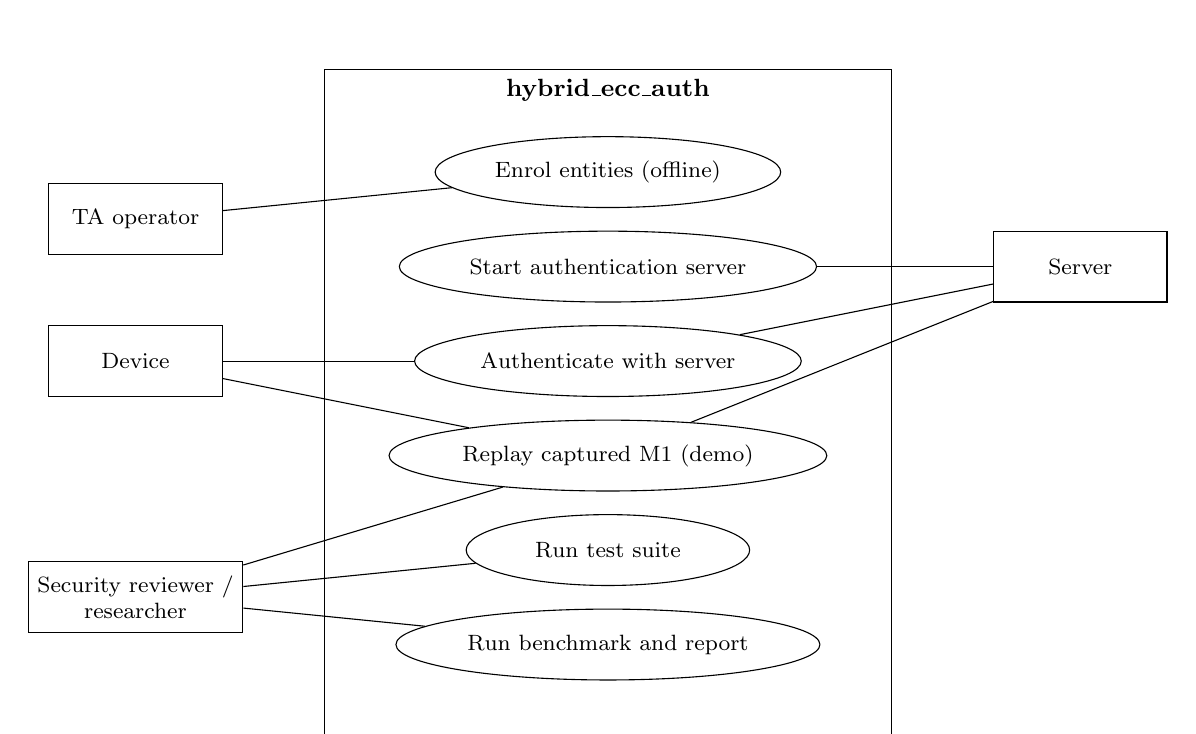
\begin{tikzpicture}
\node[draw,rectangle,minimum width=72mm,minimum height=86mm] (sys) {};
\node[anchor=north,font=\small\bfseries] at (sys.north) {hybrid\_ecc\_auth};
\node[usecase] (u1) at (0,3.0) {Enrol entities (offline)};
\node[usecase] (u2) at (0,1.8) {Start authentication server};
\node[usecase] (u3) at (0,0.6) {Authenticate with server};
\node[usecase] (u4) at (0,-0.6) {Replay captured M1 (demo)};
\node[usecase] (u5) at (0,-1.8) {Run test suite};
\node[usecase] (u6) at (0,-3.0) {Run benchmark and report};
\node[ext] (a1) at (-6,2.4) {TA operator};
\node[ext] (a2) at (-6,0.6) {Device};
\node[ext] (a3) at (6,1.8) {Server};
\node[ext] (a4) at (-6,-2.4) {Security reviewer /\\ researcher};
\draw (a1) -- (u1); \draw (a3) -- (u2); \draw (a3) -- (u3);
\draw (a2) -- (u3); \draw (a2) -- (u4); \draw (a3) -- (u4);
\draw (a4) -- (u5); \draw (a4) -- (u6); \draw (a4) -- (u4);
\end{tikzpicture}
\caption{Use-case diagram}
\label{fig:usecase}
\end{figure}

\textbf{Class diagram.} Figure~\ref{fig:class} shows the main classes. \texttt{Device} and \texttt{Server} share pairwise-root caching, coverage checking and session-key derivation through the \texttt{Entity} base class. Each owns a \texttt{SessionLog} for replay and block-list state.

\begin{figure}[H]
\centering
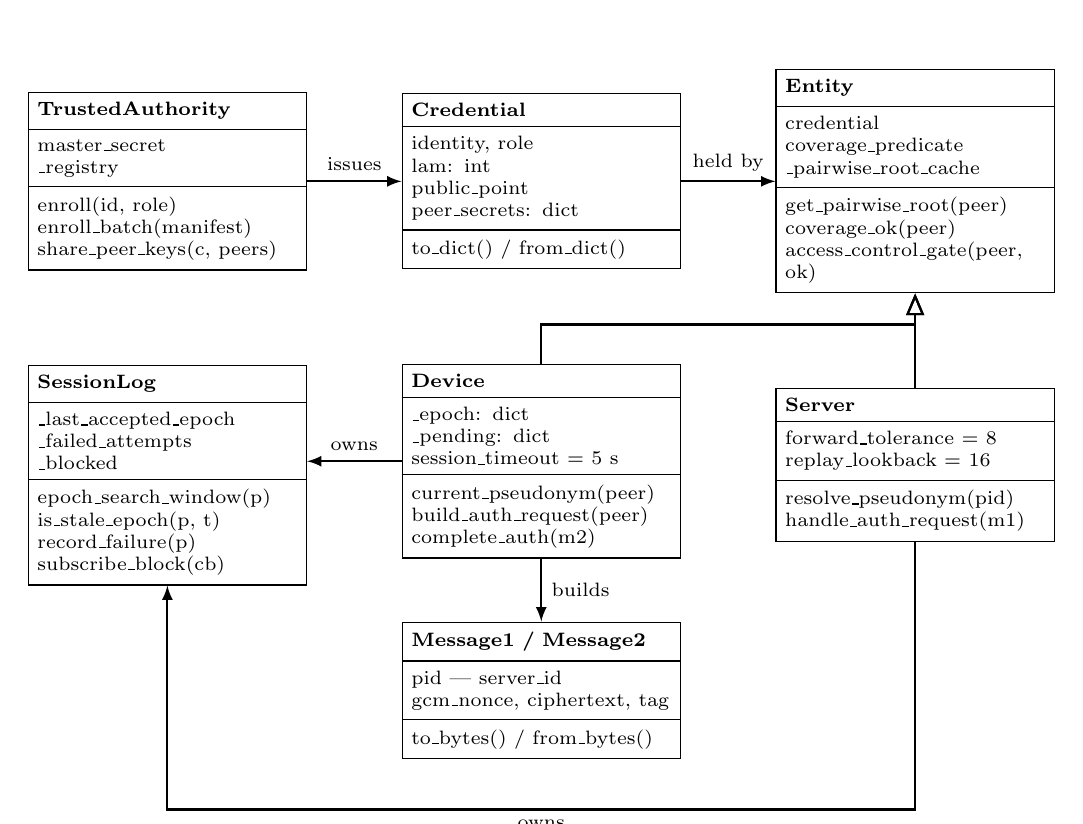
\begin{tikzpicture}[node distance=6mm and 12mm]
\node[cls] (ta) {\textbf{TrustedAuthority}\nodepart{second}master\_secret\\ \_registry\nodepart{third}enroll(id, role)\\ enroll\_batch(manifest)\\ share\_peer\_keys(c, peers)};
\node[cls,right=of ta] (cred) {\textbf{Credential}\nodepart{second}identity, role\\ lam: int\\ public\_point\\ peer\_secrets: dict\nodepart{third}to\_dict() / from\_dict()};
\node[cls,right=of cred] (ent) {\textbf{Entity}\nodepart{second}credential\\ coverage\_predicate\\ \_pairwise\_root\_cache\nodepart{third}get\_pairwise\_root(peer)\\ coverage\_ok(peer)\\ access\_control\_gate(peer, ok)};
\node[cls,below=12mm of cred] (dev) {\textbf{Device}\nodepart{second}\_epoch: dict\\ \_pending: dict\\ session\_timeout = 5 s\nodepart{third}current\_pseudonym(peer)\\ build\_auth\_request(peer)\\ complete\_auth(m2)};
\node[cls,below=12mm of ent] (srv) {\textbf{Server}\nodepart{second}forward\_tolerance = 8\\ replay\_lookback = 16\nodepart{third}resolve\_pseudonym(pid)\\ handle\_auth\_request(m1)};
\node[cls,below=12mm of ta] (log) {\textbf{SessionLog}\nodepart{second}\_last\_accepted\_epoch\\ \_failed\_attempts\\ \_blocked\nodepart{third}epoch\_search\_window(p)\\ is\_stale\_epoch(p, t)\\ record\_failure(p)\\ subscribe\_block(cb)};
\node[cls,below=8mm of dev] (m) {\textbf{Message1 / Message2}\nodepart{second}pid | server\_id\\ gcm\_nonce, ciphertext, tag\nodepart{third}to\_bytes() / from\_bytes()};
\draw[arr] (ta) -- node[above,font=\scriptsize]{issues} (cred);
\draw[arr] (cred) -- node[above,font=\scriptsize]{held by} (ent);
\draw[-open triangle 45,thick] (dev.north) -- ++(0,5mm) -| (ent.south);
\draw[-open triangle 45,thick] (srv) -- (ent);
\draw[arr] (dev.west) -- node[above,font=\scriptsize]{owns} (log.east |- dev.west);
\draw[arr] (srv.south) -- ++(0,-34mm) -| node[pos=0.25,below,font=\scriptsize]{owns} (log.south);
\draw[arr] (dev) -- node[right,font=\scriptsize]{builds} (m);
\end{tikzpicture}
\caption{Class diagram of the protocol core}
\label{fig:class}
\end{figure}

\textbf{Sequence diagram.} Figure~\ref{fig:seq} shows the complete flow: offline provisioning followed by the two-message online exchange.

\begin{figure}[H]
\centering
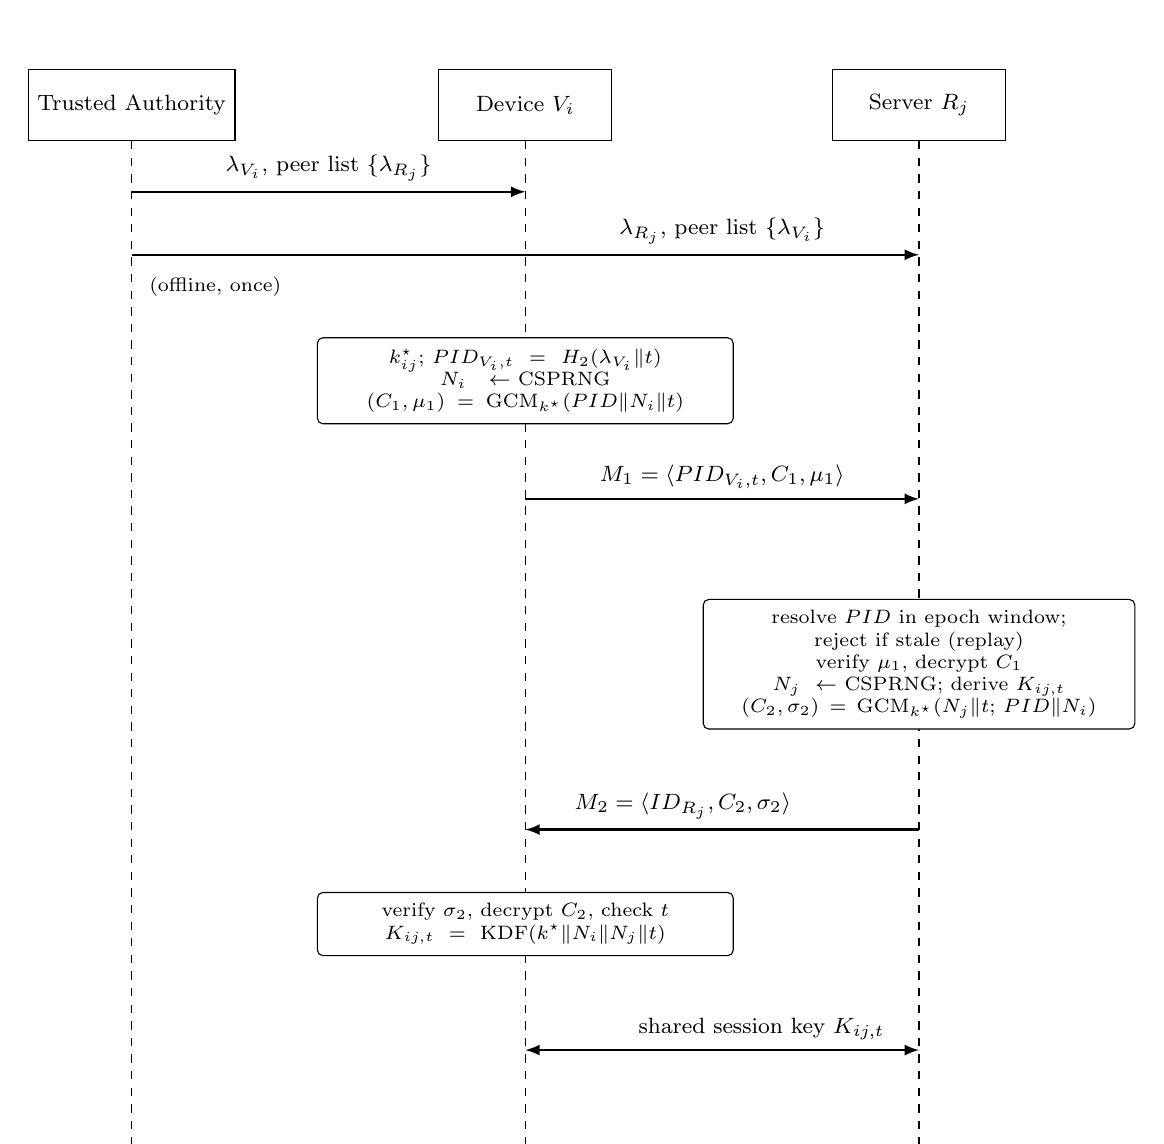
\begin{tikzpicture}[font=\footnotesize]
\node[ext] (T) at (0,0) {Trusted Authority};
\node[ext] (D) at (5,0) {Device $V_i$};
\node[ext] (S) at (10,0) {Server $R_j$};
\foreach \n in {T,D,S} \draw[dashed] (\n.south) -- ++(0,-12.9);
\draw[arr] (0,-1.1) -- node[above]{$\lambda_{V_i}$, peer list $\{\lambda_{R_j}\}$} (5,-1.1);
\draw[arr] (0,-1.9) -- node[above,pos=0.75]{$\lambda_{R_j}$, peer list $\{\lambda_{V_i}\}$} (10,-1.9);
\node[font=\scriptsize,anchor=west] at (0.1,-2.3) {(offline, once)};
\node[blk,fill=white,text width=50mm,font=\scriptsize] at (5,-3.5) {$k^\star_{ij}$; $PID_{V_i,t}=H_2(\lambda_{V_i}\|t)$\\ $N_i \leftarrow$ CSPRNG\\ $(C_1,\mu_1)=\mathrm{GCM}_{k^\star}(PID\|N_i\|t)$};
\draw[arr] (5,-5.0) -- node[above]{$M_1 = \langle PID_{V_i,t}, C_1, \mu_1\rangle$} (10,-5.0);
\node[blk,fill=white,text width=52mm,font=\scriptsize] at (10,-7.1) {resolve $PID$ in epoch window;\\ reject if stale (replay)\\ verify $\mu_1$, decrypt $C_1$\\ $N_j \leftarrow$ CSPRNG; derive $K_{ij,t}$\\ $(C_2,\sigma_2)=\mathrm{GCM}_{k^\star}(N_j\|t;\,PID\|N_i)$};
\draw[arr] (10,-9.2) -- node[above,pos=0.6]{$M_2 = \langle ID_{R_j}, C_2, \sigma_2\rangle$} (5,-9.2);
\node[blk,fill=white,text width=50mm,font=\scriptsize] at (5,-10.4) {verify $\sigma_2$, decrypt $C_2$, check $t$\\ $K_{ij,t}=\mathrm{KDF}(k^\star\|N_i\|N_j\|t)$};
\draw[latex-latex,thick] (5,-12.0) -- node[above,pos=0.6]{shared session key $K_{ij,t}$} (10,-12.0);
\end{tikzpicture}
\caption{Sequence diagram: offline registration and two-message mutual authentication}
\label{fig:seq}
\end{figure}

\subsection{Block Diagram}
\begin{figure}[H]
\centering
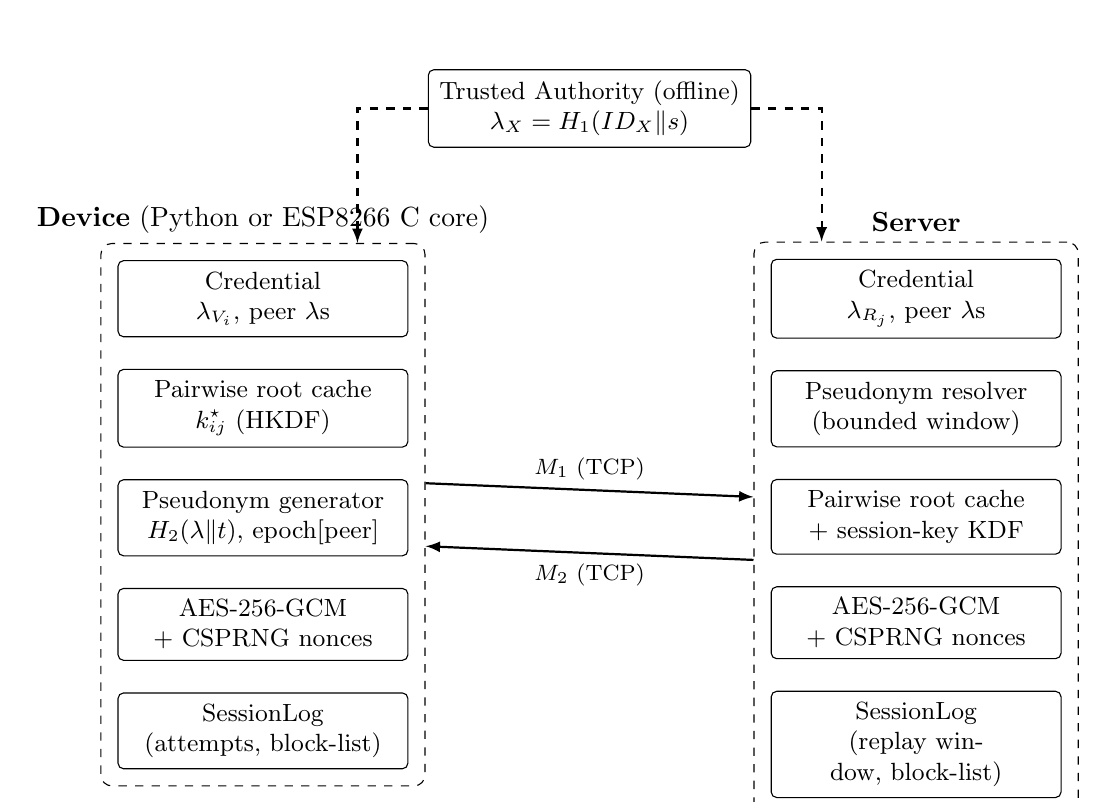
\begin{tikzpicture}[node distance=4mm]
\node[blk,text width=34mm] (dc) {Credential\\ $\lambda_{V_i}$, peer $\lambda$s};
\node[blk,text width=34mm,below=of dc] (dk) {Pairwise root cache\\ $k^\star_{ij}$ (HKDF)};
\node[blk,text width=34mm,below=of dk] (dp) {Pseudonym generator\\ $H_2(\lambda\|t)$, epoch[peer]};
\node[blk,text width=34mm,below=of dp] (da) {AES-256-GCM\\ + CSPRNG nonces};
\node[blk,text width=34mm,below=of da] (dl) {SessionLog\\ (attempts, block-list)};
\node[grp,fit=(dc)(dl),label=above:{\textbf{Device} (Python or ESP8266 C core)}] (DEV) {};
\node[blk,text width=34mm,right=46mm of dc] (sc) {Credential\\ $\lambda_{R_j}$, peer $\lambda$s};
\node[blk,text width=34mm,below=of sc] (sr) {Pseudonym resolver\\ (bounded window)};
\node[blk,text width=34mm,below=of sr] (sk) {Pairwise root cache\\ + session-key KDF};
\node[blk,text width=34mm,below=of sk] (sa) {AES-256-GCM\\ + CSPRNG nonces};
\node[blk,text width=34mm,below=of sa] (sl) {SessionLog\\ (replay window, block-list)};
\node[grp,fit=(sc)(sl),label=above:{\textbf{Server}}] (SRV) {};
\node[blk,above=12mm of $(DEV.north)!0.5!(SRV.north)$] (ta) {Trusted Authority (offline)\\ $\lambda_X = H_1(ID_X\|s)$};
\draw[arr,dashed] (ta) -| ([xshift=12mm]DEV.north);
\draw[arr,dashed] (ta) -| ([xshift=-12mm]SRV.north);
\draw[arr] ([yshift=4mm]DEV.east) -- node[above,font=\footnotesize]{$M_1$ (TCP)} ([yshift=4mm]SRV.west);
\draw[arr] ([yshift=-4mm]SRV.west) -- node[below,font=\footnotesize]{$M_2$ (TCP)} ([yshift=-4mm]DEV.east);
\end{tikzpicture}
\caption{Block diagram of the system components}
\label{fig:block}
\end{figure}

\subsection{Data Flow Diagram}
\textbf{Level 0 (context).} Figure~\ref{fig:dfd0} treats the authentication system as a single process. The manifest enters the TA, and credential bundles are written for each entity. Devices send authentication requests and receive responses, and the server writes JSON log events.

\begin{figure}[H]
\centering
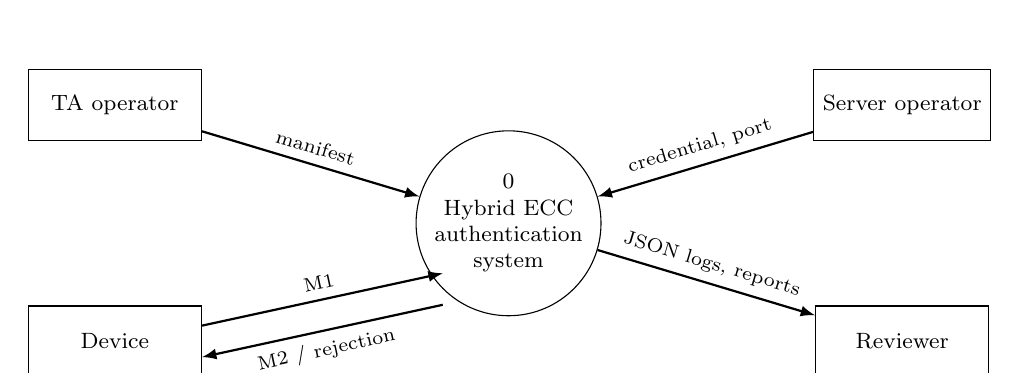
\begin{tikzpicture}
\node[proc] (p) at (0,0) {0\\ Hybrid ECC\\ authentication\\ system};
\node[ext] (op) at (-5,1.5) {TA operator};
\node[ext] (dv) at (-5,-1.5) {Device};
\node[ext] (rv) at (5,1.5) {Server operator};
\node[ext] (lg) at (5,-1.5) {Reviewer};
\draw[arr] (op) -- node[above,sloped,font=\scriptsize]{manifest} (p);
\draw[arr] ([yshift=2mm]dv.east) -- node[above,sloped,font=\scriptsize]{M1} ([yshift=2mm]p.south west);
\draw[arr] ([yshift=-2mm]p.south west) -- node[below,sloped,font=\scriptsize]{M2 / rejection} ([yshift=-2mm]dv.east);
\draw[arr] (rv) -- node[above,sloped,font=\scriptsize]{credential, port} (p);
\draw[arr] (p) -- node[above,sloped,font=\scriptsize]{JSON logs, reports} (lg);
\end{tikzpicture}
\caption{Data flow diagram, level 0}
\label{fig:dfd0}
\end{figure}

\textbf{Level 1.} Figure~\ref{fig:dfd1} breaks the system into its main processes and the data stores they read and write.

\begin{figure}[H]
\centering
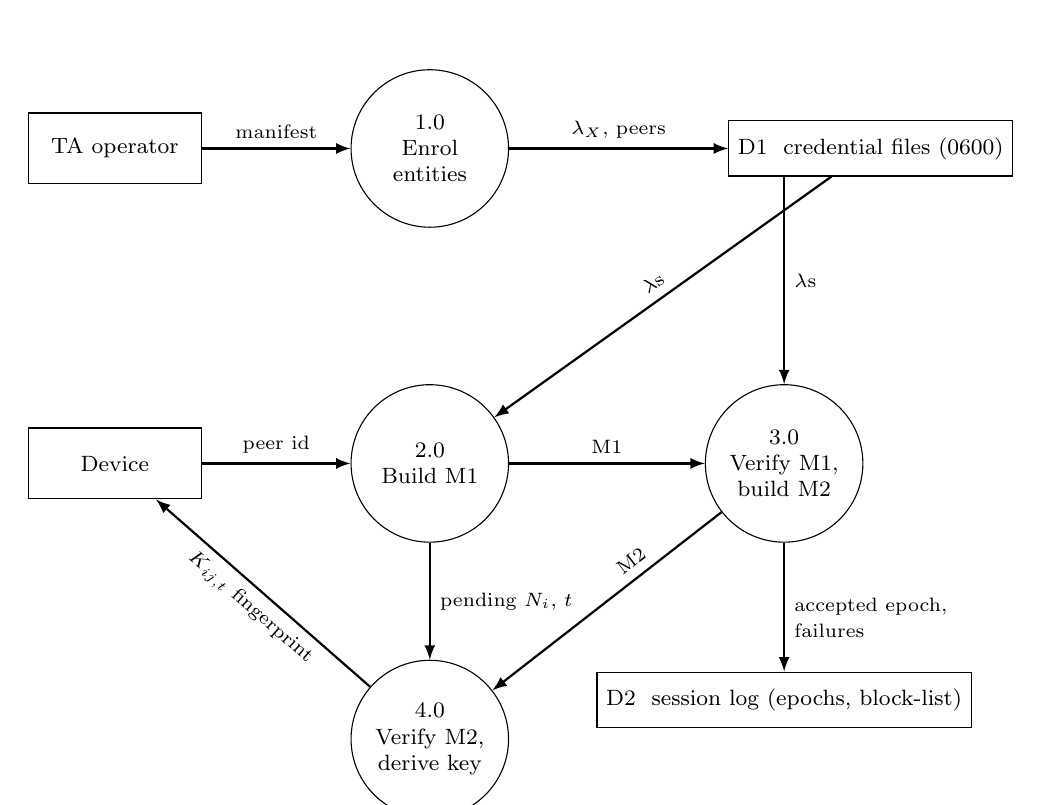
\begin{tikzpicture}
\node[ext] (op) at (-6,4) {TA operator};
\node[proc] (p1) at (-2,4) {1.0\\ Enrol\\ entities};
\node[store] (d1) at (3.6,4) {D1 \ credential files (0600)};
\node[ext] (dv) at (-6,0) {Device};
\node[proc] (p2) at (-2,0) {2.0\\ Build M1};
\node[proc] (p3) at (2.5,0) {3.0\\ Verify M1,\\ build M2};
\node[store] (d2) at (2.5,-3) {D2 \ session log (epochs, block-list)};
\node[proc] (p4) at (-2,-3.5) {4.0\\ Verify M2,\\ derive key};
\draw[arr] (op) -- node[above,font=\scriptsize]{manifest} (p1);
\draw[arr] (p1) -- node[above,font=\scriptsize]{$\lambda_X$, peers} (d1);
\draw[arr] (d1.south -| p3) -- node[right,font=\scriptsize]{$\lambda$s} (p3);
\draw[arr] (d1) -- node[above,sloped,font=\scriptsize]{$\lambda$s} (p2);
\draw[arr] (dv) -- node[above,font=\scriptsize]{peer id} (p2);
\draw[arr] (p2) -- node[above,font=\scriptsize]{M1} (p3);
\draw[arr] (p3) -- node[right,font=\scriptsize]{accepted epoch,} node[right,font=\scriptsize,yshift=-3mm]{failures} (d2);
\draw[arr] (p3) -- node[above,sloped,pos=0.35,font=\scriptsize]{M2} (p4);
\draw[arr] (p2) -- node[right,font=\scriptsize]{pending $N_i$, $t$} (p4);
\draw[arr] (p4) -- node[below,sloped,font=\scriptsize]{$K_{ij,t}$ fingerprint} (dv);
\end{tikzpicture}
\caption{Data flow diagram, level 1}
\label{fig:dfd1}
\end{figure}

\subsection{Timeline Chart}
Where the Gantt chart shows activities, Figure~\ref{fig:timeline} shows the project's milestones: dated deliverables and decision points recorded in the repository.

\begin{figure}[H]
\centering
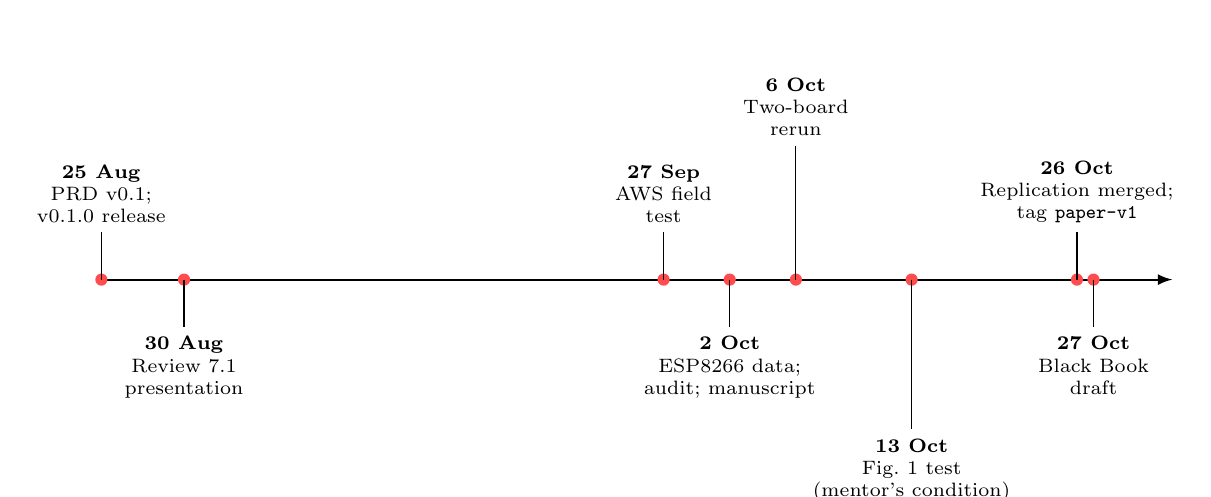
\begin{tikzpicture}[font=\scriptsize]
\draw[thick,-latex] (0,0) -- (13.6,0);
% x = (days since 25 Aug) * 0.21; y = label offset (positive above, negative below)
\foreach \x/\d/\t/\y in {
  0/25 Aug/{PRD v0.1;\\ v0.1.0 release}/0.6,
  1.05/30 Aug/{Review 7.1\\ presentation}/-0.6,
  7.14/27 Sep/{AWS field\\ test}/0.6,
  7.98/2 Oct/{ESP8266 data;\\ audit; manuscript}/-0.6,
  8.82/6 Oct/{Two-board\\ rerun}/1.7,
  10.29/13 Oct/{Fig.~1 test\\ (mentor's condition)}/-1.9,
  12.39/26 Oct/{Replication merged;\\ tag \texttt{paper-v1}}/0.6,
  12.6/27 Oct/{Black Book\\ draft}/-0.6}
{
  \fill[red!70] (\x,0) circle (2.2pt);
  \draw (\x,0) -- (\x,\y);
  \pgfmathparse{\y>0 ? 1 : 0}
  \ifnum\pgfmathresult=1
    \node[align=center,anchor=south] at (\x,\y) {\textbf{\d}\\ \t};
  \else
    \node[align=center,anchor=north] at (\x,\y) {\textbf{\d}\\ \t};
  \fi
}
\end{tikzpicture}
\caption{Project milestone timeline (2026)}
\label{fig:timeline}
\end{figure}

\section{Hardware Requirements}
Table~\ref{tab:hw} lists the hardware on which the project's results were produced, as recorded in the repository's result files and reports.

\begin{table}[H]
\centering
\caption{Hardware used for development and measurement}
\label{tab:hw}
\small
\begin{tabularx}{\textwidth}{|P{0.19\textwidth}|Y|P{0.18\textwidth}|P{0.17\textwidth}|}
\hline
\textbf{Component} & \textbf{Specification (as recorded)} & \textbf{Used for} & \textbf{Availability}\\ \hline
NodeMCU ESP8266 boards (2) & Tensilica L106, 80\,MHz (also run at 160\,MHz), about 80\,KB RAM, no cryptographic hardware; chip IDs 00d37d28 and 00d377aa & Device firmware, primitive benchmark & \MISSING{}\\ \hline
Apple-silicon laptop & Model not recorded & Primitive benchmark (BearSSL and OpenSSL), server scaling & \MISSING{}\\ \hline
Windows~11 laptop & 16 logical CPUs; WSL2 Ubuntu 22.04.5 with 7\,GB RAM & Replication study, OMNeT++ & \MISSING{}\\ \hline
Linux laptop & Intel Core i5-12500H, 16 logical CPUs, 15\,GiB RAM, kernel 6.18.57 & Re-runs for this report & \MISSING{}\\ \hline
AWS t4g.nano (2 + 1) & Graviton2 (Neoverse-N1), 2 vCPU, 512\,MiB, Amazon Linux 2023, us-east-1 & Two-node field test; primitive benchmark & Paid, on demand\\ \hline
GitHub-hosted runners & \texttt{ubuntu-latest} & CI & Free\VERIFY{}\\ \hline
\end{tabularx}
\end{table}

\noindent No 8- or 16-bit microcontroller, MCU with cryptographic hardware, or energy-measurement equipment was used. \MISSING{Whether each laptop and the ESP8266 boards are personally owned or institute-provided, and the minimum specification, if the department requires one.}

\section{Software Requirements}
\begin{table}[H]
\centering
\caption[Software requirements]{Software requirements (versions from \texttt{pyproject.toml}, lock files and result logs)}
\label{tab:sw}
\small
\begin{tabularx}{\textwidth}{|P{0.25\textwidth}|Y|P{0.22\textwidth}|}
\hline
\textbf{Item} & \textbf{Purpose} & \textbf{Version}\\ \hline
Python & Reference implementation, audit and replication scripts & $\ge$3.11 (3.11.9, 3.11.16, 3.14.8 used)\\ \hline
\texttt{cryptography} (OpenSSL) & P-256, HKDF-SHA256, AES-256-GCM in Python & 50.0.0 / 50.0.1\\ \hline
pytest, pytest-cov, hypothesis & Unit, property and coverage testing & 9.1.1, 7.1.0, 6.165.10\\ \hline
matplotlib, numpy & Charts and analysis & 3.11.x, 2.4--2.5\\ \hline
C compiler, Make & Native build of the C device core and benchmark & --\\ \hline
BearSSL (ESP8266 fork) & AES-GCM, SHA, HKDF, P-256 in C & as shipped with the ESP8266 Arduino core\\ \hline
PlatformIO, Arduino core for ESP8266 & Firmware build and flashing (\texttt{espressif8266}, \texttt{nodemcuv2}) & --\\ \hline
OpenSSL libcrypto & Hardware-accelerated primitive comparison on the laptop & --\\ \hline
OMNeT++ & Network model of the paper's Table~II setting & 6.0.3 (Academic Public License)\\ \hline
SimPy, PyMuPDF, PyYAML & Cross-check simulation; PDF rendering; data extraction & 4.1.2, 2.0, 6.0.3\\ \hline
Docker, Docker Compose & Multi-node IoT emulation and benchmark runner & --\\ \hline
AWS CLI, Amazon Linux 2023 & Cloud field test & AL2023.12\\ \hline
Git, GitHub Actions & Version control and CI (Python 3.11, 3.12) & --\\ \hline
LaTeX & Manuscript and report & --\\ \hline
\end{tabularx}
\end{table}

\section{Cost Estimation}
\label{sec:cost}
\begin{table}[H]
\centering
\caption{Cost estimation}
\label{tab:cost}
\small
\begin{tabularx}{\textwidth}{|>{\centering\arraybackslash}p{0.055\textwidth}|P{0.18\textwidth}|Y|P{0.2\textwidth}|}
\hline
\textbf{Sr. No.} & \textbf{Item / Resource} & \textbf{Description} & \textbf{Estimated Cost (Rs.)}\\ \hline
1 & Hardware & Laptops (Table~\ref{tab:hw}); 2 NodeMCU ESP8266 boards & \MISSING{laptops existing? board price}\\ \hline
2 & Software / Tools & All tools in Table~\ref{tab:sw} are free or open source; project released under Apache-2.0 & 0 (free/open-source)\\ \hline
3 & Cloud / Hosting & AWS t4g.nano at US\$0.0042/h each (2 nodes for the field test plus 1 for benchmarking) and 2 $\times$ 8\,GB gp3 volumes; instances terminated after use. Public GitHub repository and Actions & \MISSING{actual AWS bill; GitHub 0?}\\ \hline
4 & APIs / Services & None & 0\\ \hline
5 & Other Expenses & Base paper via the institute's IEEE Xplore subscription (existing resource) & \MISSING{printing, binding, publication fees}\\ \hline
 & \textbf{Total Estimated Cost} & & \MISSING{}\\ \hline
\end{tabularx}
\end{table}

All software is free or open source, and no paid API is used. The only recurring cost was the AWS instances, which the field-test report prices at US\$0.0042 per hour each, plus storage. Since the instances ran only for the duration of the tests, the bill depends on how long they ran, which is not recorded. The ESP8266 boards are the only hardware bought specifically for the project, if they were bought.

\section{Conclusion}
The methodology has four stages: implement the base paper's Section~III protocol in Python and in C for an ESP8266; measure the primitives of the paper's cost model on three hardware classes with one benchmark source; audit the paper's tables, equations and figures; and recompute its comparison under four readings of the proposed scheme's cost, with an OMNeT++ model used only for sensitivity analysis. Requirements come from the PRD and the review cycle, and are expressed as eight functional and seven non-functional requirements. A documented epoch window fills a gap in the paper's specification. The layered architecture separates primitives, protocol, storage, demonstration and benchmarking, so the protocol core can be ported, as the ESP8266 firmware shows. Hardware and software needs are modest and mostly free, with small cloud and board costs. This methodology produces the implementation and evidence presented in Chapter~4.

\ChapterDivider{Implementation \& Results}
\chapter{Implementation \& Results}
\section{Introduction}
This chapter describes what was built and what it produced. The implementation has five parts: the Python reference implementation; the C device core and ESP8266 firmware; a two-node cloud deployment; the primitive benchmark and paper-audit scripts; and the replication pipeline with its OMNeT++ model. Five aspects are evaluated: functional correctness, security behaviour, end-to-end operation on three kinds of platform, the measured cost of the primitives and of the protocol, and the base paper's claims recomputed with that evidence. Results marked \emph{re-run} were regenerated for this report on the Linux laptop in Table~\ref{tab:hw}; their raw outputs are in \path{blackbook/run_outputs/}. All other results are the team's committed measurements, with their source file named.

\section{Implementation}
\textbf{Code base.} Table~\ref{tab:loc} summarises the repository.

\begin{table}[H]
\centering
\caption{Implementation components (lines include comments)}
\label{tab:loc}
\small
\begin{tabularx}{\textwidth}{|P{0.33\textwidth}|c|c|Y|}
\hline
\textbf{Component} & \textbf{Files} & \textbf{Lines} & \textbf{Contents}\\ \hline
\path{hybrid_ecc_auth/crypto/} & 5 & 181 & P-256, $H_1/H_2/H_3$, HKDF, AES-GCM, nonces\\ \hline
\path{hybrid_ecc_auth/protocol/} & 8 & 706 & TA, Entity, Device, Server, messages, login gate, errors, rekey stub\\ \hline
\path{hybrid_ecc_auth/storage/} & 2 & 154 & Replay window, block-list, keystore\\ \hline
\path{hybrid_ecc_auth/demo/} & 4 & 432 & TCP framing, \texttt{hea-ta}, \texttt{hea-server}, \texttt{hea-device}\\ \hline
\path{hybrid_ecc_auth/bench/} & 4 & 968 & Cost model, paper reference data, harness, report\\ \hline
\path{hybrid_ecc_auth/tests/} & 15 & 1{,}385 & Unit, property, adversarial\\ \hline
\path{firmware/esp8266/} (core, firmware) & 3 & 474 & Portable C protocol core, Arduino firmware\\ \hline
\path{firmware/esp8266/} (bench, host, tools) & 7 & 534 & Primitive benchmark, native build, interop tools\\ \hline
\path{research/paper_audit/} & 12 & 656 & Audit, recomputation, protocol checks\\ \hline
\path{research/reference_replication/} & 27 & 3{,}944 & Replication scripts, OMNeT++ model, tests\\ \hline
\end{tabularx}
\end{table}

\textbf{Python reference implementation.} Each cryptographic primitive is a thin wrapper over the \texttt{cryptography} library. $\lambda_X$ is SHA-256 of identity and master secret reduced modulo the P-256 order. AES-GCM uses a fresh 96-bit IV per message and returns the 16-byte tag separately so that it can serve as $\mu_1$ or $\sigma_2$. Listing~\ref{lst:m1} shows the core of $M_1$ construction. The plaintext layout, $PID$ (32~B) $\|$ $N_i$ (16~B) $\|$ $t$ (8~B), is an implementation choice, because the paper does not specify byte layouts.

\begin{lstlisting}[language=Python,caption={Building $M_1$ (excerpt from \texttt{protocol/device.py})},label={lst:m1}]
k_star = self.get_pairwise_root(peer_id)
epoch = self._epoch.get(peer_id, 0)
pid = self.current_pseudonym(peer_id, epoch)
n_i = generate_nonce(self.nonce_bits)

plaintext = pid + n_i + epoch.to_bytes(8, "big")
gcm_nonce, ciphertext, tag = aead.encrypt(k_star, plaintext)
msg1 = Message1(pid=pid, gcm_nonce=gcm_nonce, ciphertext=ciphertext, tag=tag)
\end{lstlisting}

On the server, the block-list check runs before any decryption, and the response binds $PID\|N_i$ as additional authenticated data (Listing~\ref{lst:m2}).

\begin{lstlisting}[language=Python,caption={Building $M_2$ (excerpt from \texttt{protocol/server.py})},label={lst:m2}]
self.session_log.accept_epoch(peer_identity, epoch)
self.session_log.record_success(peer_identity)

n_j = generate_nonce(self.nonce_bits)
session_key = derive_session_key(k_star, n_i, n_j, epoch)

aad = msg1.pid + n_i
plaintext2 = n_j + epoch.to_bytes(8, "big")
gcm_nonce2, ciphertext2, tag2 = aead.encrypt(k_star, plaintext2, aad=aad)
\end{lstlisting}

Messages are compact JSON with base64-encoded fields and a version number. The demo transport adds a 4-byte length prefix and a success/error envelope. \texttt{hea-ta enroll} reads a manifest, enrols every entity, cross-issues peer keys and writes credential files with mode 0600. \texttt{hea-server} serves requests and logs one JSON event per attempt. \texttt{hea-device} prints a fingerprint of the session key, never the key itself, and \texttt{--replay-last} resends the previous $M_1$. The benchmark harness measures message sizes, processing time (1{,}000 warm and 100 cold trials) and persisted-state size, and sweeps server cost from 100 to 1{,}800 enrolled devices. GitHub Actions runs the tests with a 90\% coverage gate on Python 3.11 and 3.12. A Docker Compose setup runs a multi-node emulation and the benchmark.

\textbf{C device core and ESP8266 firmware.} \path{firmware/esp8266/lib/hea_proto} is a portable C port of the device side on BearSSL \cite{bearssl} (AES-256-GCM, SHA-256, HKDF-SHA256), with no Arduino dependencies. It produces the identical framed-JSON wire format, so it talks to the unmodified Python server. \path{src/main.cpp} adds Wi-Fi, a handshake loop, per-step timings and a replay test. Unlike the Python reference, the firmware persists the epoch to flash. Offline enrolment stays on the laptop, and the board receives only $\lambda_{device}$ and $\lambda_{server}$. The same core builds natively, and \path{tools/interop.py} checks it against the Python server without hardware.

\textbf{Primitive benchmark.} \path{firmware/esp8266/bench/prim_bench.c} is the single C source used on every platform. On the ESP8266 it runs with Wi-Fi off and cycle-counter timing; P-256 runs on a temporary heap stack because the 4\,KB task stack is too small. \path{research/paper_audit/libcrypto_bench.c} times OpenSSL \cite{openssl} with hardware AES and SHA on the laptop, per message, with a low-level HKDF verified equal to OpenSSL's.

\textbf{Audit and recomputation scripts.} \path{research/paper_audit/} contains the table transcription with OCR verification (\texttt{paper\_tables.py}, \texttt{verify\_tables.py}), the consistency audit (\texttt{audit.py}), figure digitisation (\texttt{figures\_audit.py}), the recomputation with measured constants (\texttt{reeval.py}, \texttt{eq22\_variants.py}), the Fig.~1 test (\texttt{fig1\_repro.py}), and the forward-secrecy and server-scaling checks.

\textbf{Replication pipeline.} \path{research/reference_replication/} reproduces the three comparator papers' own numbers, audits how the base paper used them, compares all schemes under three sets of constants (the base paper's, the comparator papers' own, and the measured ones), and runs a network simulation of the base paper's Table~II setting. The simulation is an OMNeT++ 6.0.3 \cite{omnetpp} model written by the team, because the base paper publishes no simulation files, cross-checked against an independent SimPy model. The pipeline reports 46 passing tests, and its OMNeT++ sweep (3{,}385 runs) is byte-identical when repeated. \VERIFY{The replication suite needs PyYAML, SimPy and PyMuPDF, which are not installed in this environment, so its tests were not re-run for this report.}

\textbf{Cloud deployment.} On 27 September 2026 the Python implementation was deployed on two AWS t4g.nano instances (device node and server node) in one availability zone. The repository's own scripts ran there: the test suite, CLI walkthrough, handshake loops, security scenarios over the network, and the full benchmark.

\textbf{Traceability.} Table~\ref{tab:trace} maps the paper's symbols to code.

\begin{table}[H]
\centering
\caption{Paper symbol to code traceability}
\label{tab:trace}
\small
\begin{tabularx}{\textwidth}{|P{0.22\textwidth}|c|Y|}
\hline
\textbf{Paper symbol} & \textbf{Eq.} & \textbf{Code reference}\\ \hline
$\lambda_X$ & 8 & \path{protocol/ta.py :: derive_long_term_secret}\\ \hline
$k^\star_{ij}$ & 9 & \path{protocol/entity.py :: derive_pairwise_root}\\ \hline
$cov_{ij}(t)$ & 10 & \path{protocol/entity.py :: Entity.coverage_ok}\\ \hline
$PID_{V_i,t}$ & 11 & \path{protocol/device.py :: Device.current_pseudonym}\\ \hline
$N_i, C_1, \mu_1, M_1$ & 12--15 & \path{protocol/device.py :: Device.build_auth_request}\\ \hline
$K_{ij,t}$ & 16 & \path{protocol/entity.py :: derive_session_key}\\ \hline
$\sigma_2, C_2, M_2$ & 17--19 & \path{protocol/server.py :: Server.handle_auth_request}\\ \hline
Correctness & 20 & \path{tests/property/test_session_key_agreement.py}\\ \hline
$Allow_{ij}(t)$ & 23 & \path{protocol/entity.py :: Entity.access_control_gate}\\ \hline
Rekey & 24 & \path{protocol/rekey.py} (stub)\\ \hline
\end{tabularx}
\end{table}

\section{Results of Implementation}
\label{sec:results}

\subsection*{Functional and adversarial tests (re-run)}
After pulling the latest repository, the test suite ran 108 tests: 97 unit, 2 property-based and 9 adversarial (SEC-03 runs twice). All passed. The property test ran 10{,}000 randomised sessions with zero key mismatches. Line coverage of \path{protocol/} and \path{crypto/} is 97\% (Table~\ref{tab:cov}). The same suite also passed on the AWS device node (108 passed in 10.8\,s, 97\% coverage).

\begin{table}[H]
\centering
\caption{Line coverage of \texttt{protocol/} and \texttt{crypto/}}
\label{tab:cov}
\small
\begin{tabular}{|l|r|r|r|}
\hline
\textbf{Module} & \textbf{Statements} & \textbf{Missed} & \textbf{Coverage}\\ \hline
\path{crypto/} (5 modules) & 67 & 1 & 99\%\\ \hline
\path{protocol/device.py} & 71 & 4 & 94\%\\ \hline
\path{protocol/server.py} & 62 & 3 & 95\%\\ \hline
\path{protocol/messages.py} & 54 & 3 & 94\%\\ \hline
\path{protocol/ta.py} & 47 & 1 & 98\%\\ \hline
other \path{protocol/} modules & 65 & 0 & 100\%\\ \hline
\textbf{Total} & \textbf{366} & \textbf{12} & \textbf{97\%}\\ \hline
\end{tabular}
\end{table}

\begin{table}[H]
\centering
\caption{Adversarial test cases (PRD Section~7.2), all passing}
\label{tab:sec}
\small
\begin{tabularx}{\textwidth}{|P{0.09\textwidth}|Y|Y|}
\hline
\textbf{ID} & \textbf{Scenario} & \textbf{Expected and observed result}\\ \hline
SEC-01 & Replay a captured valid $M_1$ & Rejected: stale epoch\\ \hline
SEC-02 & Replay a captured $M_2$ into another session & Rejected: $\sigma_2$/nonce binding\\ \hline
SEC-03 & Flip one bit in $C_1$ or $\mu_1$ & Rejected: tag verification (both cases)\\ \hline
SEC-04 & Forge $M_1$ for a known PID without $\lambda_{V_i}$ & Rejected: invalid $\mu_1$\\ \hline
SEC-05 & Three consecutive failures & Block-listed; 4th attempt rejected before any cryptography\\ \hline
SEC-06 & Compare pseudonyms across epochs & Indistinguishability smoke test passes\\ \hline
SEC-07 & Two independent honest runs & Different session keys\\ \hline
SEC-08 & Out-of-coverage device & Rejected at $Allow_{ij}(t)$\\ \hline
\end{tabularx}
\end{table}

\subsection*{End-to-end demonstration on one machine (re-run)}
\begin{lstlisting}[numbers=none,basicstyle=\ttfamily\scriptsize,caption={CLI demo output: enrolment, successful authentication, replay rejection and server log},label={lst:demo}]
$ hea-ta enroll --manifest manifest.json --out-dir creds/
Enrolled 'device-001' (role=device) -> creds/device-001.json
Enrolled 'server-A' (role=server) -> creds/server-A.json
2 entities enrolled and cross-issued peer keys. Offline phase complete -- no network I/O occurred.

$ hea-device authenticate --credential creds/device-001.json --server-id server-A --server-addr 127.0.0.1:18443
Mutual authentication succeeded with 'server-A'.
  session key fingerprint: e1507ce5d2d12bcf (SHA-256[:16] of K_ij,t -- never the raw key)
  round-trip latency: 4.218 ms

$ hea-device authenticate ... --replay-last
[replay-demo] resending previously captured M1 (216 bytes) to 127.0.0.1:18443 ...
REJECTED by server: ReplayDetected: pseudonym for 'device-001' reuses stale epoch 0 (round-trip 2.286 ms)

server log:
{"event": "auth_attempt", "outcome": "accepted", "peer_identity": "device-001", "latency_ms": 1.5397, ...}
{"event": "auth_attempt", "outcome": "rejected", "error_type": "ReplayDetected", ..., "latency_ms": 0.0884, ...}
\end{lstlisting}

\subsection*{ESP8266 device against the Python server}
The C device core completed 12 of 12 handshakes natively and 20 of 20 on a NodeMCU ESP8266 over Wi-Fi against the unmodified Python server. In every case the session-key fingerprints on both sides were identical, and a replayed $M_1$ was rejected. On the ESP8266 at 80\,MHz, building $M_1$ took 1.67~ms and verifying $M_2$ and deriving the key took 3.59~ms: 5.26~ms of device computation per handshake (mean of 20), and 52~ms end to end over Wi-Fi. $M_1$ is 216~bytes. \VERIFY{These figures are as reported in the team's manuscript; the raw handshake log is not committed, and the native interop check was not re-run because building it requires downloading BearSSL.}

\subsection*{Two-node cloud field test}
\begin{table}[H]
\centering
\caption{AWS t4g.nano field test (device and server on separate instances; 2{,}000 handshakes, 0 failures, 2{,}000 unique session keys)}
\label{tab:aws}
\small
\begin{tabular}{|l|r|r|r|}
\hline
\textbf{Segment (ms)} & \textbf{p50} & \textbf{p95} & \textbf{p99}\\ \hline
Device: build $M_1$ & 0.041 & 0.057 & 0.070\\ \hline
Network round trip incl.\ server & 0.617 & 0.804 & 0.917\\ \hline
Device: verify $M_2$ + KDF & 0.067 & 0.100 & 0.131\\ \hline
End-to-end handshake & 0.728 & 0.931 & 1.059\\ \hline
Server \texttt{handle\_auth\_request} (server log) & 0.132 & 0.163 & 0.194\\ \hline
\end{tabular}
\end{table}
\noindent About two-thirds of a handshake was TCP round trip. Sequential throughput was 1{,}326 handshakes/s. Messages were 216~B ($M_1$) and 136~B ($M_2$), 409~B of TCP payload with framing. The device process peaked at 30~MB of memory. Source: \path{docs/experiments/aws_demo_2026-09-27/}.

\subsection*{Protocol cost on a laptop (re-run)}
\begin{table}[H]
\centering
\caption{Measured message sizes per session}
\label{tab:comm}
\small
\begin{tabular}{|l|P{0.42\textwidth}|r|r|}
\hline
\textbf{Message} & \textbf{Raw fields (bytes)} & \textbf{Raw total} & \textbf{JSON wire}\\ \hline
$M_1$ & PID 32, IV 12, ciphertext 56, tag 16 & 116 & 216\\ \hline
$M_2$ & server ID 14, IV 12, ciphertext 24, tag 16 & 66 & 142\\ \hline
\textbf{Session} & & \textbf{182 (1{,}456 bits)} & \textbf{358}\\ \hline
\end{tabular}
\end{table}
\noindent The $M_2$ size depends on the server identifier: 14 characters here, 8 (\texttt{server-A}) in the AWS test.

\begin{table}[H]
\centering
\caption{Measured processing time per session on the Linux laptop (ms)}
\label{tab:proc}
\small
\begin{tabular}{|l|r|r|r|r|}
\hline
\textbf{Operation} & \textbf{Trials} & \textbf{Mean} & \textbf{Median} & \textbf{p95}\\ \hline
Device total (warm) & 1000 & 0.047 & 0.039 & 0.090\\ \hline
Server: handle $M_1$ (warm) & 1000 & 0.073 & 0.061 & 0.143\\ \hline
Device total (cold) & 100 & 0.047 & 0.047 & 0.053\\ \hline
Server total (cold) & 100 & 0.067 & 0.068 & 0.072\\ \hline
\end{tabular}
\end{table}
\noindent Persisted state is 424~bytes for a device and 449~bytes for a server with one peer each. Figure~\ref{fig:comm} compares the measured message size with the paper's reported values for the other schemes.

\begin{figure}[H]
\centering
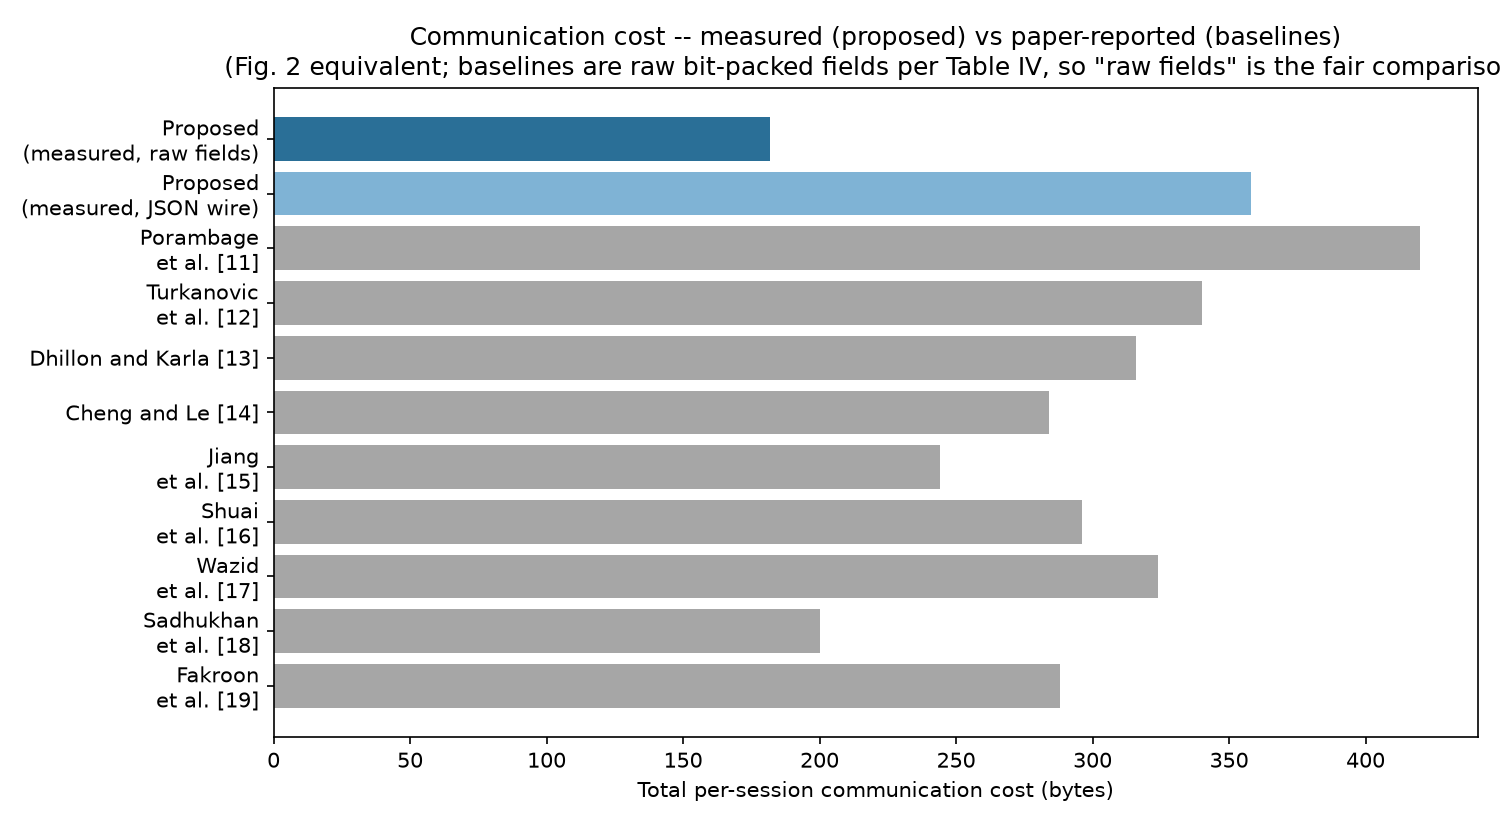
\includegraphics[width=0.95\textwidth]{figures/communication_cost.png}
\caption{Communication cost: measured (proposed) vs.\ paper-reported baselines (Table~IV)}
\label{fig:comm}
\end{figure}

\subsection*{Measured primitive costs}
\begin{table}[H]
\centering
\caption{Paper constants vs.\ measured medians (GCM: 56-byte AES-256-GCM including key setup, \texttt{aes\_big}/\texttt{aes\_ct})}
\label{tab:constants}
\small
\begin{tabular}{|l|r|r|r|r|}
\hline
 & \textbf{Paper} & \textbf{ESP8266} & \textbf{ESP8266} & \textbf{Graviton2}\\
 & \textbf{(Table III)} & \textbf{80\,MHz} & \textbf{160\,MHz} & \textbf{t4g.nano}\\ \hline
$T_H$ (SHA-1) & 0.32\,ms & 36\,$\mu$s & 18\,$\mu$s & 0.23\,$\mu$s\\ \hline
$T_{SE/D}$ (GCM) & 5.6\,ms & 0.48/1.15\,ms & 0.24/0.57\,ms & 2.0/6.9\,$\mu$s\\ \hline
$T_{ECM}$ (P-256) & 17.1\,ms & 276\,ms & 138\,ms & 1.75\,ms\\ \hline
HKDF-SHA256 & -- & 629\,$\mu$s & 315\,$\mu$s & 3.2\,$\mu$s\\ \hline
$T_{ECM}/T_H$ & 53 & 7{,}600 & 7{,}600 & 7{,}700\\ \hline
\end{tabular}
\end{table}
\noindent Source: \path{research/paper_audit/results/*.csv}. All benchmark outputs are checksummed: the 41 digests are identical on all BearSSL platforms. On the ESP8266 the 25th and 75th percentiles equal the median, and a rerun on a second board (6 October 2026) reproduced every median exactly. On the laptop, absolute times shifted by 1.3--2.3$\times$ in Low Power Mode, so only ratios are used from it.

\subsection*{Protocol-level checks (re-run)}
\begin{itemize}[nosep]
  \item \textbf{Forward secrecy:} an attacker who later obtains $k^\star$ recovered 5 of 5 past session keys from recorded $M_1$/$M_2$ alone.
  \item \textbf{Server lookup:} resolving a pseudonym took 0.47, 4.81 and 23.85~ms on the Apple-silicon laptop at 100, 1{,}000 and 5{,}000 devices, using a 13-epoch window (committed result). On the Linux laptop the same script measured 1.80, 19.86 and 77.57~ms at 100, 1{,}000 and 5{,}000 devices. In the AWS test, server cost grew by about 13~$\mu$s per enrolled device, reaching 26.1~ms at 1{,}800 devices.
\end{itemize}

\section{Result Analysis}
\textbf{Implementation objectives.} All five implementation objectives were met: 97\% coverage against a 90\% target; 10{,}000 correctness trials with no failures; a working three-terminal demo with a correctly classified replay rejection; all eight SEC cases passing; and a median authentication time of about 0.1~ms, against a 5~ms budget. The measurement objectives were also met: the device side runs on an ESP8266 and interoperates with the Python server, and the primitives were measured on three hardware classes.

\textbf{Consistency of the paper's evidence.} Table~\ref{tab:audit} summarises the audit (re-run with \texttt{audit.py}, \texttt{figures\_audit.py} and \texttt{fig1\_repro.py}; outputs match the committed results).

\begin{table}[H]
\centering
\caption{Consistency audit of the base paper}
\label{tab:audit}
\small
\begin{tabularx}{\textwidth}{|P{0.06\textwidth}|P{0.3\textwidth}|Y|}
\hline
\textbf{\#} & \textbf{Finding} & \textbf{Evidence}\\ \hline
A1 & 17/21/12\% not derivable & None of nine definitions gives these values within one point. Table~IV: 36.0\% vs best, 57.5\% vs mean. Table~VI: 10.1\% (device) and 33.3\% (server) vs best. Figures: 24--49\%, 19--31\%, 7--25\%.\\ \hline
A2 & Tables contradict text & Table~IV: 4 messages, 1{,}024 bits. Text and Eq.~21: 2 messages, 264 bits, yet $2\times128 = 256$, and a SHA-256 pseudonym plus a GCM tag already exceed 264 bits in $M_1$ alone.\\ \hline
A3 & Not the cheapest under its own constants & Table~V $\times$ Table~III: proposed 23.68~ms (device + server); Turkanovi\'{c} 3.84, Dhillon--Kalra 4.48, ``Jiang'' 4.80~ms.\\ \hline
A4 & Internal inconsistencies & Table~V charges $2T_H+2T_{SE/D}$, Eq.~22 one KDF, one encryption and one MAC. Algorithms~1--2 describe a different protocol. Table~VI is captioned ``communication''. Two schemes share reference [17]. ``5\% (one per hundred devices)''.\\ \hline
A5 & Figures disagree with text & Fig.~1 captioned processing, axis communication. Figs.~1--2 plot ``vehicles in VANET''. Fig.~2's per-session bit cost rises with vehicles. The figures compare against four schemes cited nowhere in the paper.\\ \hline
A6 & Row labels do not match references & ``Cheng and Le [14]'', ``Jiang [15]'', ``Shuai [16]'' point to Wang \emph{et al.}, Wen \emph{et al.}\ and the chaotic-map Jiang paper. ``Cheng--Le'' matches Chang and Le's P2 with counts exchanged. Turkanovi\'{c}'s device and server counts are swapped.\\ \hline
A7 & Constants differ from source papers & $T_C$: 0.32~ms in the base paper vs 32.40~ms in Jiang \emph{et al.}; $T_{ECM}$: 17.1 vs 63.075~ms in Chang and Le.\\ \hline
\end{tabularx}
\end{table}

\textbf{Fig.~1 could not be reproduced.} The paper gives no simulation scenario, code or data, and two web searches found none, so the simulation is \emph{not publicly available}. The paper's own cost method gives a per-authentication cost independent of the number of vehicles, but the digitised Fig.~1 curves rise by 5--21 units. A flat fit leaves residuals of 10--36 times the reading error, and even an affine fit leaves the proposed curve at 20 times. This shows only that Fig.~1 depends on undocumented simulation effects, not that it is wrong. The team's own OMNeT++ model of the Table~II setting (Figure~\ref{fig:omnet}) depends on guessed inputs (adversary rate, arrival window, which devices a server must resolve, server class). The proposed scheme's mean latency at 1{,}000 devices ranges from about 2~ms to 5.6~s across those guesses, so the model is used only as a sensitivity analysis.

\begin{figure}[H]
\centering
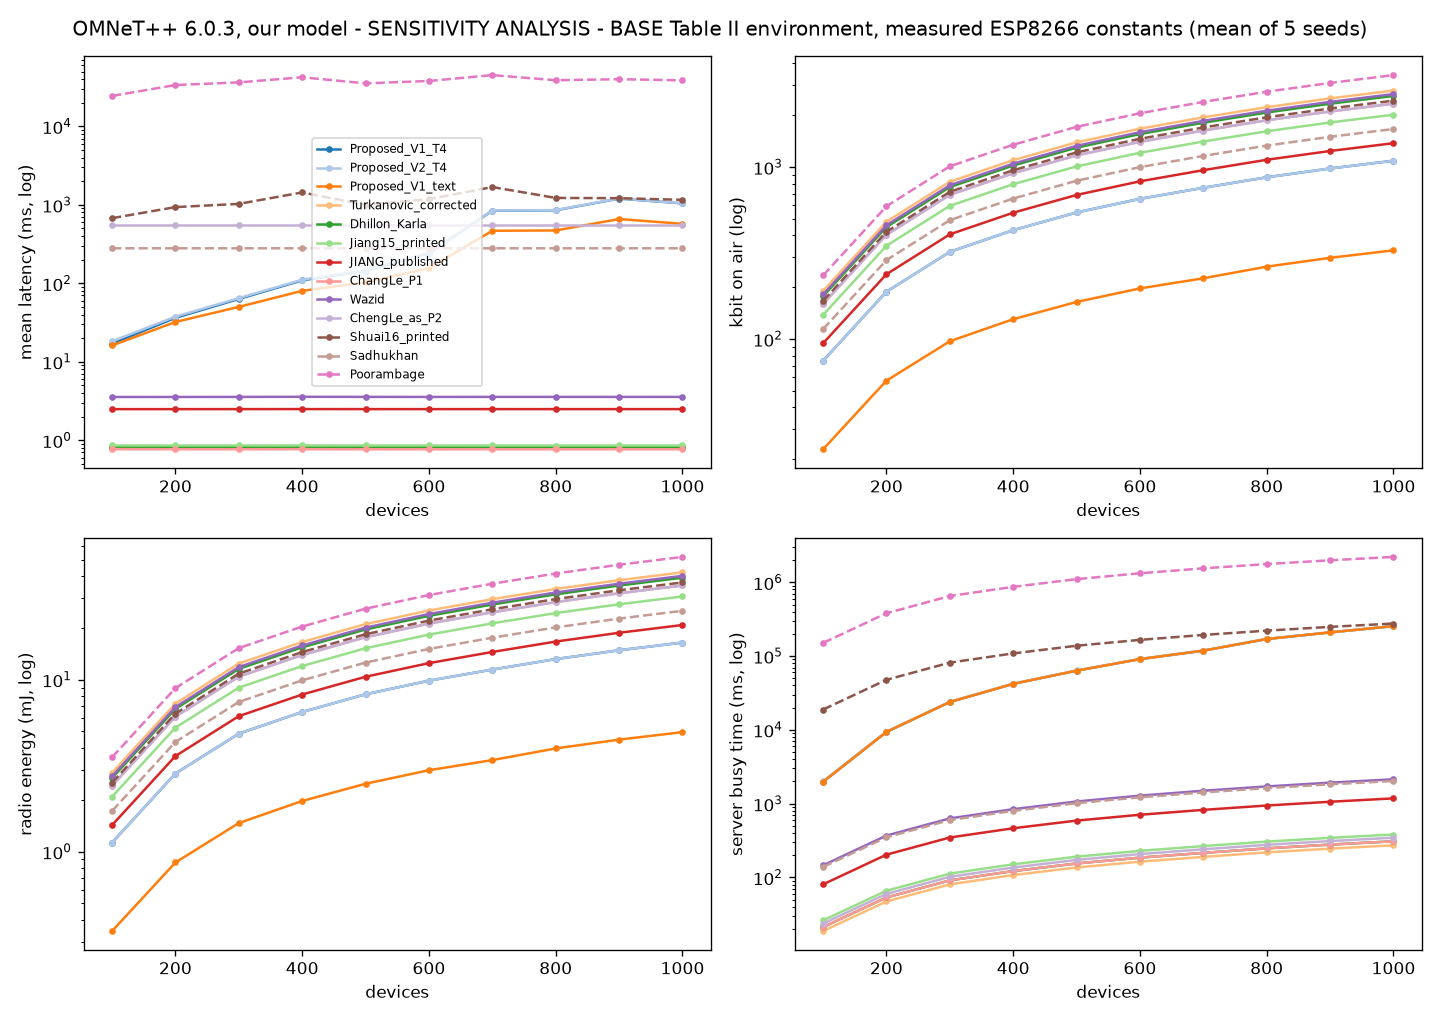
\includegraphics[width=\textwidth]{figures/step5b_omnet_meas.png}
\caption{OMNeT++ sensitivity analysis of the base paper's Table~II setting with measured ESP8266 constants (team's model; mean of 5 seeds)}
\label{fig:omnet}
\end{figure}

\textbf{Recomputed ranking against ECC-based schemes.} With measured ESP8266 constants (80\,MHz, device + server, \texttt{aes\_big}/\texttt{aes\_ct}), the proposed scheme costs 2.1/4.7~ms. Sadhukhan, Shuai and ``Cheng--Le'' cost 279--553~ms, Challa 2{,}487~ms and Porambage 5{,}251~ms, so the proposed scheme is about 60 to 2{,}500 times cheaper. Because a P-256 multiplication is 16 times slower than the paper assumes, the advantage over ECC schemes is far larger than the paper reports.

\textbf{Recomputed ranking against hash-only schemes.} Table~\ref{tab:variants} counts how many of the three hash-only rows (Turkanovi\'{c}, Dhillon--Kalra, ``Jiang'') cost less than the proposed scheme. Measured HKDF costs 6--17 $T_H$ on every platform, more than the hash-only schemes' entire device columns (5--7 $T_H$). Once the session KDF the paper's own equations require is counted (V2--V4), all three hash-only rows are cheaper in every column on every platform, including OpenSSL with hardware AES and SHA. On the ESP8266 the gap is 3.8--13.7$\times$. The conclusion is firm for Turkanovi\'{c} and Dhillon--Kalra, whose counts are confirmed by independent papers. For ``Jiang'' it holds to the extent that the survey counts for the two-factor scheme are right. The chaotic-map scheme of Jiang \emph{et al.}, with its own $T_C = 32.40$~ms, costs about 195~ms on the ESP8266 and is far dearer than the proposed scheme.

\begin{table}[H]
\centering
\caption{Hash-only rows of Table~V cheaper than the proposed scheme (device + server; GCM, cached key, \texttt{aes\_big}; re-run with \texttt{eq22\_variants.py})}
\label{tab:variants}
\small
\begin{tabular}{|l|c|c|c|c|}
\hline
\textbf{Platform} & \textbf{V1} & \textbf{V2} & \textbf{V3} & \textbf{V4}\\ \hline
ESP8266, 80 and 160\,MHz (BearSSL) & 3/3 & 3/3 & 3/3 & 3/3\\ \hline
Graviton2 t4g.nano (BearSSL) & 3/3 & 3/3 & 3/3 & 3/3\\ \hline
Laptop, BearSSL software & 3/3 & 3/3 & 3/3 & 3/3\\ \hline
Laptop, OpenSSL hardware AES/SHA & 1/3 & 3/3 & 3/3 & 3/3\\ \hline
\end{tabular}
\end{table}

\begin{figure}[H]
\centering
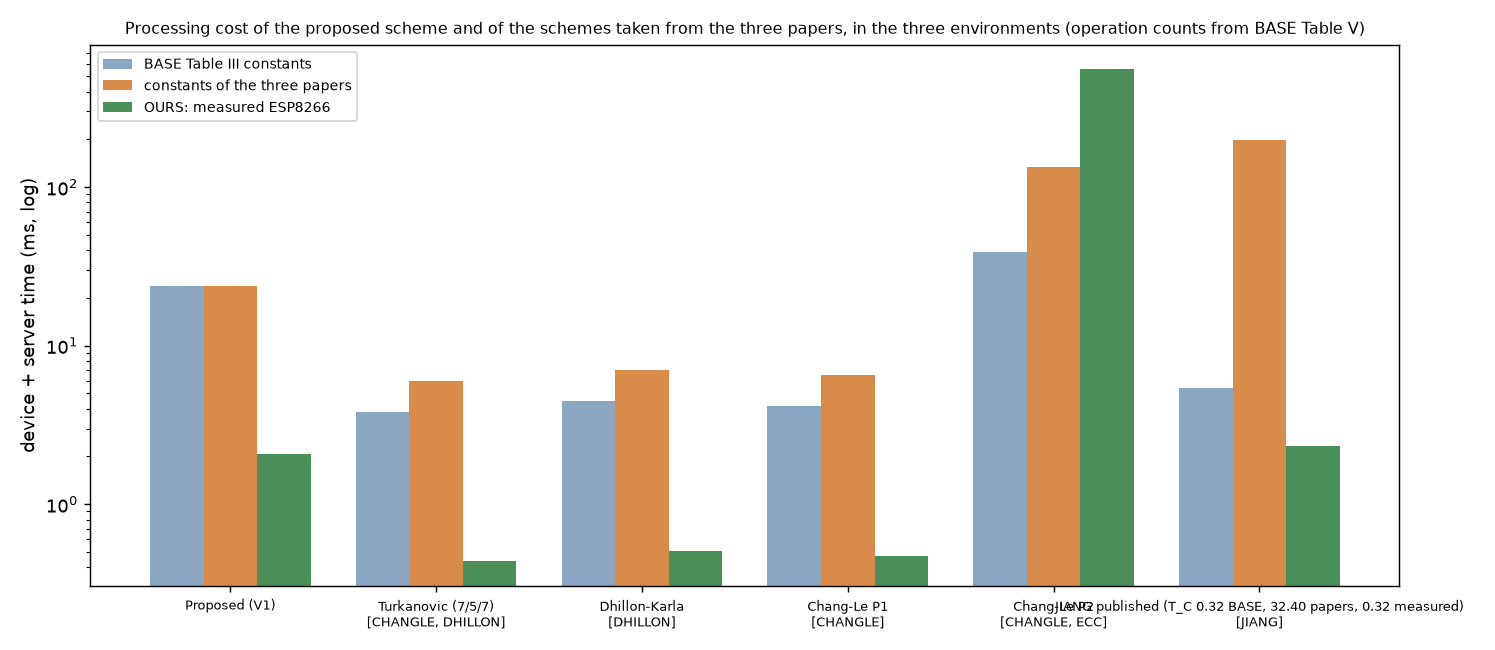
\includegraphics[width=\textwidth]{figures/step7_environments.png}
\caption{Processing cost (device + server, log scale) of the proposed scheme and the comparator schemes under the base paper's constants, the comparator papers' own constants, and measured ESP8266 constants (team's replication)}
\label{fig:env}
\end{figure}

\textbf{Communication and storage.} Against the paper's reported values, the measured 182~bytes of protocol fields is 39.6\% below the mean of Table~IV's baselines, and the team's network model also gives the proposed scheme the fewest bits on air in every variant. The direction of the communication claim therefore holds, but the magnitude cannot be checked, because the paper's own figures disagree (1{,}024 vs 264 bits). Table~VI's storage arithmetic reproduces (10.1\% and 33.3\%), but not 12\%. The 320-bit server storage also holds only if the server keeps no per-device pseudonym table; a precomputed table at 1{,}000 devices needs about 416~KB.

\textbf{Laptop measurement vs.\ the paper.} The benchmark report's ``99.9\% processing reduction'' compares 0.1~ms measured on a laptop with the paper's embedded-hardware constants. It is not meaningful and is not used as a result. The ratio-based recomputation above replaces it.

\section{Observation/Remarks}
\label{sec:obs}
\begin{itemize}
  \item \textbf{The protocol itself is light.} On an ESP8266 a whole handshake costs 5.26~ms of computation, about 52 times less than a single P-256 multiplication on the same chip. The paper's weakness is its evidence and constants, not the design idea.
  \item \textbf{ECC is nominal.} $\lambda_X$ is a hash reduced modulo $n$; the public point is optional and unused by Eq.~9--22. No elliptic-curve operation occurs online.
  \item \textbf{No forward secrecy.} Compromise of $k^\star$ exposes every past session key, unlike ECC schemes such as Chang and Le's P2.
  \item \textbf{Server cost is $O(\text{devices}\times\text{window})$.} Unlinkable pseudonyms cannot be indexed, so the server probes every device's epoch window. The paper's Table~V treats server cost as constant.
  \item \textbf{Weaknesses of the implementation found in the field test.} (i) The device epoch lives only in memory: a restarted device is rejected as a replay, or locked out after many sessions (1{,}020 of 1{,}020 retries failed after 2{,}020 sessions). The ESP8266 firmware avoids this by persisting the epoch to flash. (ii) \texttt{hea-ta enroll} distributes keys as a full mesh, so one device's credential file was enough to impersonate another device (\texttt{impersonate.py} succeeded). (iii) The block-list and replay window are lost on server restart: a blocked device authenticated again, and a pre-restart $M_1$ was accepted once (without yielding a session key). These are flaws in this implementation, not in the paper.
  \item \textbf{The operation-count model under-predicts real cost.} It gives 2.4~ms of device computation on the ESP8266, against 5.26~ms measured, because it omits HKDF, JSON/base64 parsing and per-message key scheduling.
  \item \textbf{A transcription error remains in the benchmark code.} \path{bench/baselines/reference_data.py} still lists the proposed scheme's server cost as $4T_H+5T_{ECM}$ (should be $2T_H+2T_{SE/D}$) and Sadhukhan's server cost as $2T_H+4T_{ECM}$ (should be $2T_H+4T_{SE/D}$). The audit scripts use the correct values in \path{research/paper_audit/paper_tables.py}.
  \item \textbf{Earlier claims were corrected.} An \texttt{openssl speed} proxy that suggested hardware crypto would reverse the ranking was withdrawn as not like-for-like. The team's replication also corrected the manuscript's range against ECC schemes from ``120--3{,}000$\times$'' to 60--2{,}520$\times$.
\end{itemize}

\section{Conclusion}
The base paper's Section~III protocol was implemented in Python and, on the device side, in C for an ESP8266, and the two interoperate. The implementation passes all 108 tests, runs between two cloud instances at 0.73~ms per handshake, and costs 5.26~ms of computation on a microcontroller. Using this implementation and a cross-platform primitive benchmark, the project found that: the paper's headline percentages cannot be derived from its own data; its Fig.~1 cannot be reproduced from published information; its assumed constants are off by 16$\times$ (ECC) and 5--12$\times$ (symmetric) on a real microcontroller; the scheme is 60--2{,}500$\times$ cheaper than ECC-based schemes but more expensive than the verified hash-only schemes once its own session KDF is counted; and it lacks forward secrecy and has a server lookup cost that grows with the number of devices. The field test also exposed three implementation weaknesses that a deployment would have to fix. Chapter~5 summarises the limitations and future work.

\ChapterDivider{Conclusion}
\chapter{Conclusion}
\section{Limitations}
\begin{itemize}
  \item \textbf{Not production software.} There is no HSM or secure element, no formal verification (ProVerif or Tamarin), no penetration test and no side-channel hardening. The key store relies on file permissions only.
  \item \textbf{Implementation weaknesses not yet fixed.} The Python device epoch is not persisted. TA enrolment distributes keys as a full mesh, which allows device-to-device impersonation. The server's block-list and replay window do not survive a restart. Pseudonym lookup is linear in the number of devices.
  \item \textbf{No forward secrecy, static devices, single TA.} These limitations are inherited from the base scheme. Rekeying (Eq.~24) and revocation are not implemented.
  \item \textbf{One microcontroller class.} Only a 32-bit ESP8266 was measured. There is no 8- or 16-bit part, no MCU with AES or SHA hardware, and no energy measurement.
  \item \textbf{One library family.} Primitive costs are BearSSL's and OpenSSL's; other libraries, or a hardware HKDF/HMAC engine, would shift the constants.
  \item \textbf{Competitors modelled, not run.} Comparator costs are the base paper's operation counts multiplied by measured times. The ``Jiang'' and ``Shuai'' rows were traced only through secondary tables, and no storage entry could be checked. $T_C$ and $T_{fe}$ were not measured.
  \item \textbf{Simulation is a sensitivity analysis.} The OMNeT++ model is the team's own and uses guessed inputs. It says nothing definitive about the base paper's figures.
  \item \textbf{Transcription limits.} Tables were transcribed from rendered PDFs (Table~V by hand), and figure values were read by eye. The authors of the base paper were not contacted.
\end{itemize}

\section{Conclusion}
This project set out to turn a published but unimplemented hybrid ECC mutual authentication protocol for IoT into working software, and then to test the paper's claims against it. The protocol was implemented in Python following the paper's secure, nonce-based Section~III model, and its device side was ported to C and run on an ESP8266 against the unmodified Python server. All implementation objectives were met: 108 passing tests with 97\% coverage, 10{,}000 correct key agreements, all eight adversarial cases, and working demonstrations on a laptop, two cloud nodes and a microcontroller. Measuring the primitives on real hardware showed that the paper's cost model rests on constants that are wrong in both directions. An ECC scalar multiplication is sixteen times slower than assumed, and symmetric operations are five to twelve times faster. As a result, the scheme beats ECC-based schemes by far more than the paper claims, but loses to verified hash-only schemes once the session-key derivation required by its own equations is counted. The paper's headline percentages cannot be derived from its own data, and its simulation cannot be reproduced from published information. The scheme also lacks forward secrecy and has a server lookup cost that grows with the number of devices. The protocol design is light and practical; what the project corrects is the evidence used to rank it.

\section{Future Scope}
\begin{itemize}
  \item Obtain the base paper's simulation scenario from its authors and rerun Fig.~1 against it.
  \item Measure an MCU with hardware AES and SHA, an 8/16-bit part and a Raspberry Pi~3, including energy.
  \item Read the original Shuai \emph{et al.}\ and two-factor Jiang \emph{et al.}\ papers to confirm the secondary tabulations, and verify the remaining Table~IV--VI entries.
  \item Implement and time Turkanovi\'{c} \emph{et al.}\ end to end on the microcontroller instead of modelling it.
  \item Fix the implementation weaknesses: persist the device epoch, give devices only server secrets, persist the server's block-list and replay window, and replace the linear pseudonym scan with an index of expected next pseudonyms.
  \item Complete the TA-assisted rekeying and key-revocation extension; consider an optional ephemeral key exchange for forward secrecy and measure its cost (one P-256 multiplication is 276~ms on the ESP8266).
  \item Model the Section~III message flow in Tamarin or ProVerif.
  \item Correct the transcription error in \path{bench/baselines/reference_data.py}.
\end{itemize}

% ==================== REFERENCES ====================
\clearpage
\addcontentsline{toc}{chapter}{References}
\bibliographystyle{IEEEtran}
\bibliography{references}

% ==================== APPENDIX ====================
% The appendix headings below follow the supplied index.
\chapter*{Appendix}
\addcontentsline{toc}{chapter}{Appendix}

\section*{1. Paper Details}
\addcontentsline{toc}{section}{1. Paper Details}
The team has written an IEEE conference-format manuscript from this work (\path{paper/main.tex}, release tag \texttt{paper-v1}, 26 October 2026) \cite{kerkar2026audit}.

\noindent\textbf{Title:} Do the Numbers Hold on Real Hardware? A Reproducibility and Measurement Audit of a Low-Cost Hybrid ECC Authentication Protocol for IoT\\
\textbf{Authors:} Jay Kerkar, Chaitanya Kelkar, Chirag Poornamath, Yash Kolekar; Dr.\ Shanta Sondur (Project Guide), Department of Information Technology, VESIT, Mumbai\\
\textbf{Code and data:} \url{https://github.com/jaykerkar0405/hybrid-ecc-iot-auth}

\begin{itemize}
  \item \textbf{Paper published:} \MISSING{submission status, venue/conference, acceptance or publication date, DOI/link -- the repository records only the manuscript}
  \item \textbf{Certificate of publication:} \MISSING{attach if applicable}
  \item \textbf{Plagiarism report:} \MISSING{attach the department-required report}
\end{itemize}

\section*{2. Competition certificates}
\addcontentsline{toc}{section}{2. Competition certificates}
\MISSING{No competition participation or certificates are recorded in the repository. Attach if applicable, or confirm this section should state ``Not applicable''.}

\end{document}
